\chapter{Results}
%Figure \ref{fig:cpd_perf}, shows accuracy and detection time as a function of the
%false positive rate per second, for the OSU Hip dataset,
%for each of the SVM, Decision Tree, and Neural Net base classifiers.
%
%\begin{figure}
% \centering
% 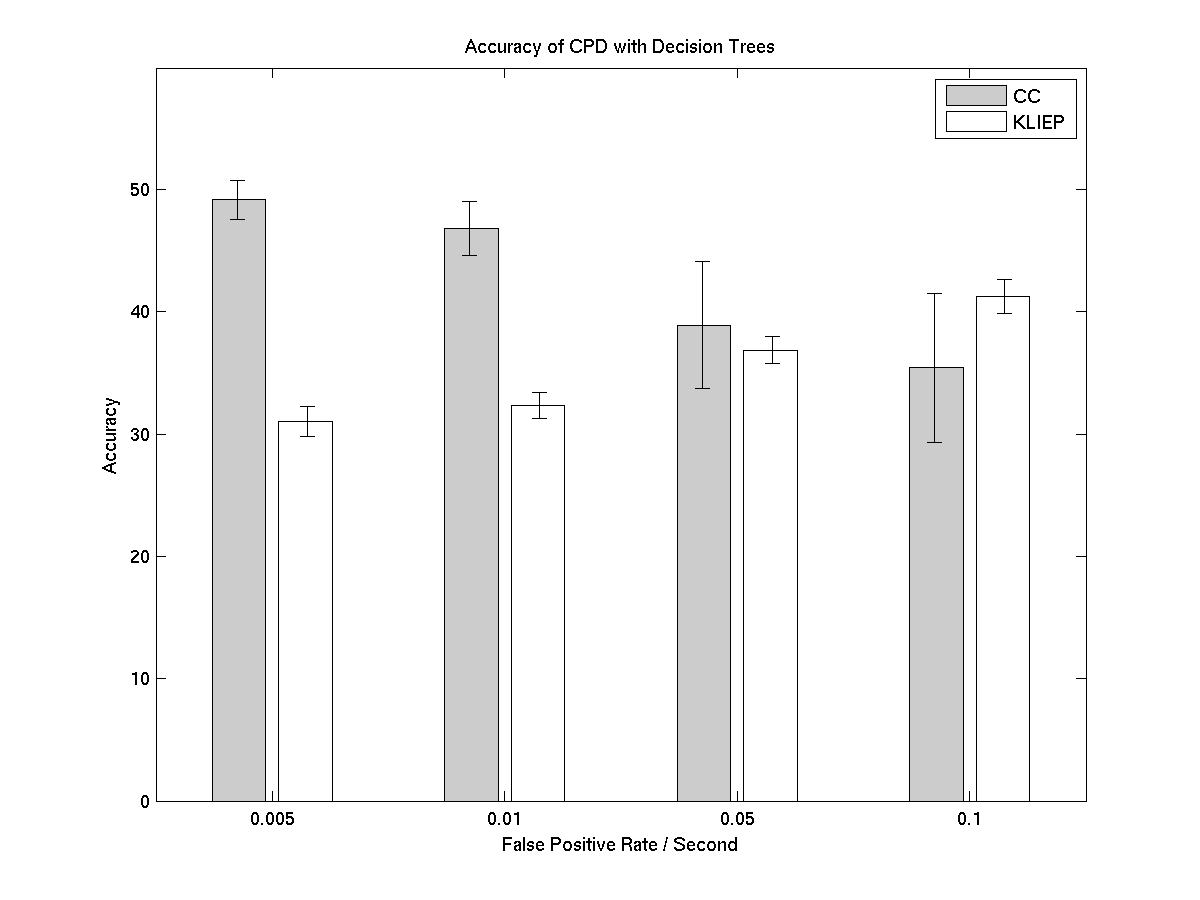
\includegraphics[scale=0.3]{osu_cpd_dt_acc.png}
% 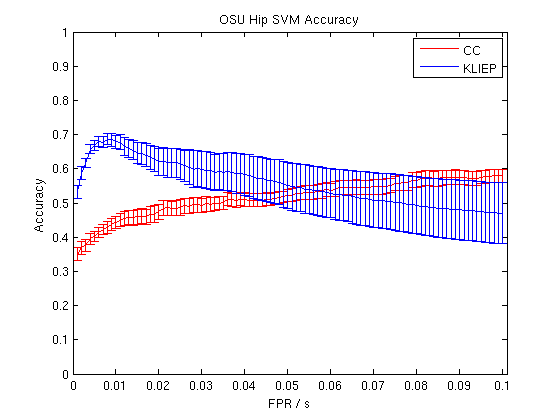
\includegraphics[scale=0.3]{osu_cpd_svm_acc.png}
% 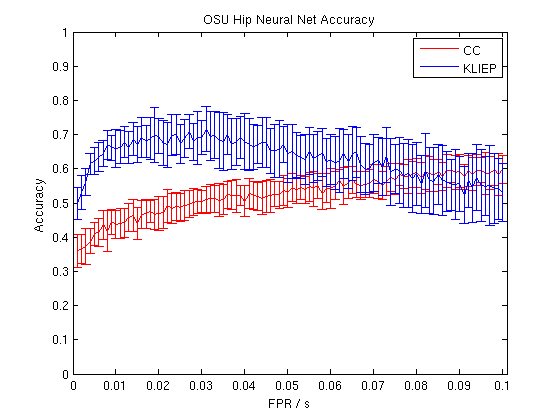
\includegraphics[scale=0.3]{osu_cpd_nnet_acc.png}
% 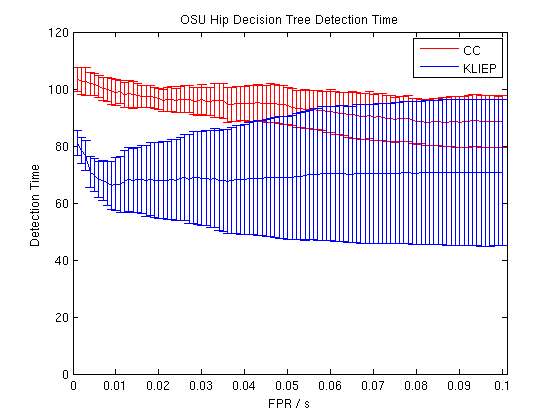
\includegraphics[scale=0.3]{osu_cpd_dt_det.png}
% 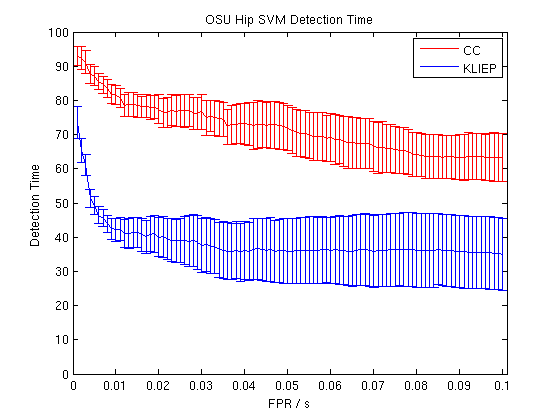
\includegraphics[scale=0.3]{osu_cpd_svm_det.png}
% 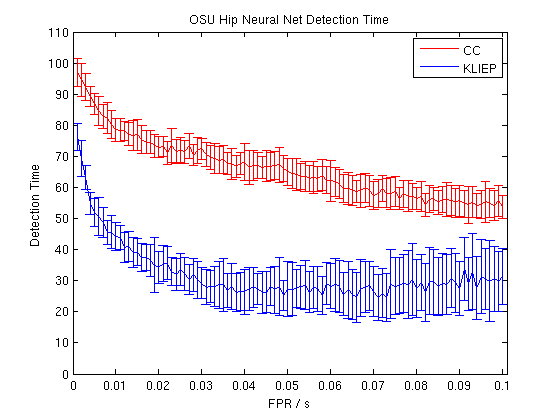
\includegraphics[scale=0.3]{osu_cpd_nnet_det.png}
% \caption{CPD-Based Classification Performance}
% \label{fig:cpd_perf}
%\end{figure}

\section{Change-Point Detection}
Results for our change-point detection experiments are given in
Figures \ref{fig:osu_cpd}-\ref{fig:lime2_cpd}.
We hypothesized that the performance of the change-point detection algorithms
would depend heavily on the threshold level for change prediction. This was
tested by varying the average number of times per second that the algorithms
falsely predicted a change. A large number of such false positive rates per
second were tested, but for the sake of brevity only a representative sample
of $\{0.005, 0.01, 0.05, 0.1\}$ are shown here.

In the OSU Hip experiments, control charts outperformed KLIEP in terms of
detection time (Figures 4.1.2, 4.1.4, 4.1.6), while the accuracy results 
(Figures 4.1.1, 4.1.3, 4.1.5) were
mixed. Except when predicted windows are large enough to span across multiple
true activities, it is generally expected that accuracy will decrease as false
positive rate increases because small windows contain less information and are
less discriminative than larger windows. This behavior is seen in the control chart
accuracy results (grey bars in Figures 4.1.1, 4.1.3, 4.1.5), but not in the
KLIEP accuracy results (white bars in Figures 4.1.1, 4.1.3, 4.1.5).
Follow-up experiments showed that KLIEP peaks in accuracy for
false positive rates between $0.2$ and $0.3$ for all three classifiers.
KlIEP seemed to perform best on this dataset when it was given many
opportunities to predict changes.

Further investigation indicated that across the OSU Hip dataset the KLIEP algorithm
was unable to detect many of the different activity changes without a very low score
threshold value (and a very high false positive rates).
Some qualitative plotting of the OSU Hip data showed
that most of its activities have accelerometer amplitude values that strongly
resemble draws from a multivariate normal distribution. Since control charts
assume that the data is drawn from a distribution that is a member of that
family, it is logical that control charts would outperform algorithms with
different modeling assumptions on OSU Hip.

In the LiME experiments, KLIEP outperformed control charts in terms of
accuracy across the board, and control charts outperformed KLIEP in terms of
detection time across the board. This suggests that in general control charts
correctly detected true changes more quickly, but that after a correct change
prediction it was more likely to make an incorrect change prediction.

In a few cases (Figures 4.1.2, 4.1.6, 4.2.6) the detection time did
not decrease as the false positive rate increased. On the face of it this would seem
to be a non-sequitur, but this only happened in cases when accuracy also decreased
(Figures 4.1.1, 4.1.5, 4.2.5).
Smaller window sizes tend to be correlated with decreased detection times, but
it is possible that predicting with smaller windows, if they happen to contain
an insufficient amount of discriminative data,
can actually increase the time required for the classifier to start correctly
predicting the ground-truth activity. Additionally, the given increases in detection
time were small and within confidence bounds.

\begin{figure}[H]
 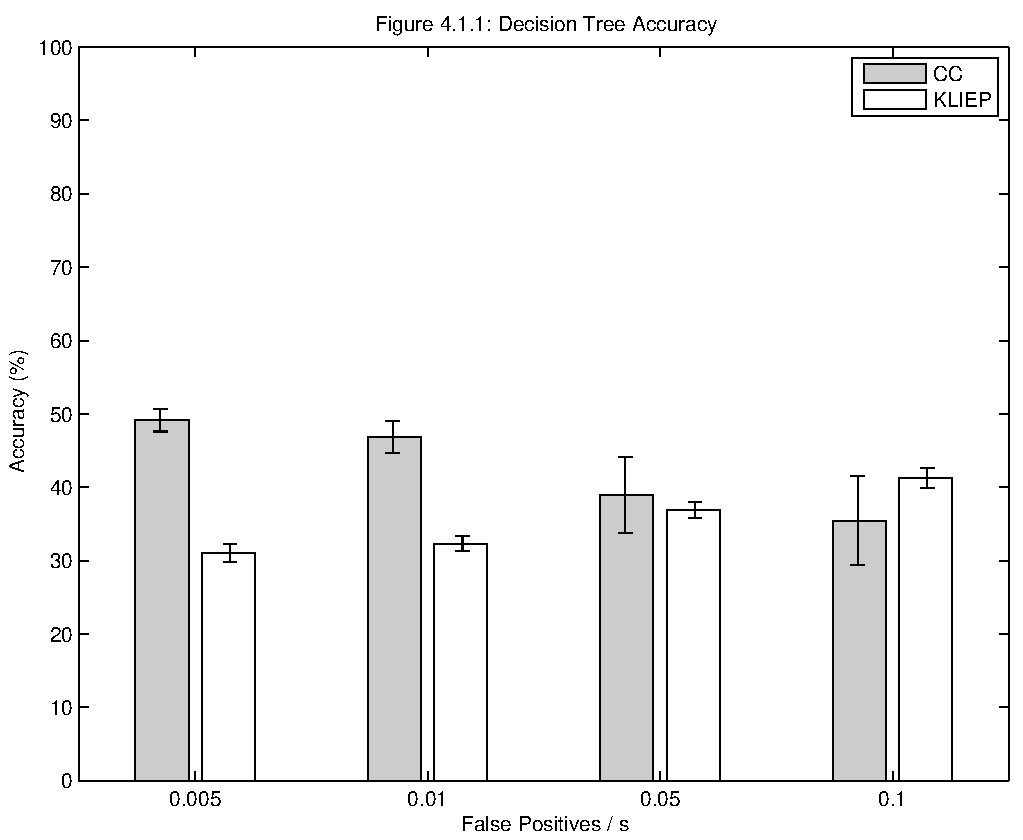
\includegraphics[scale=0.4]{osu_cpd_dt_acc.pdf} \hspace{1em}\vspace{1em}
 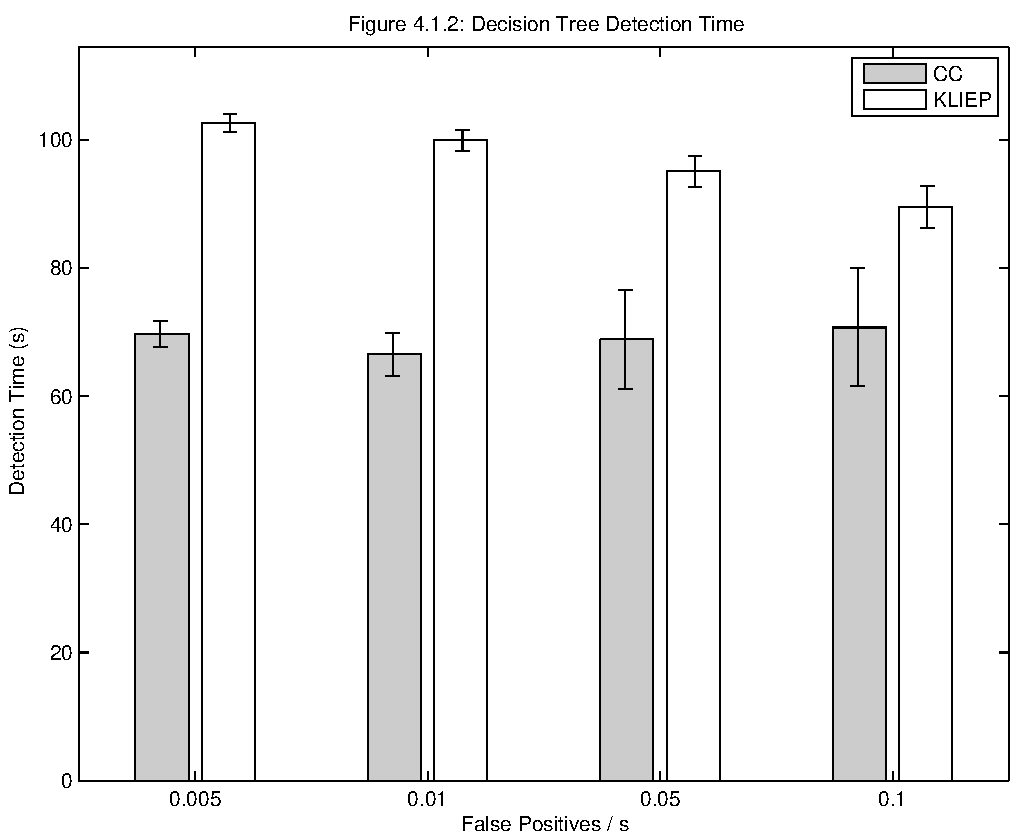
\includegraphics[scale=0.4]{osu_cpd_dt_det.pdf}
 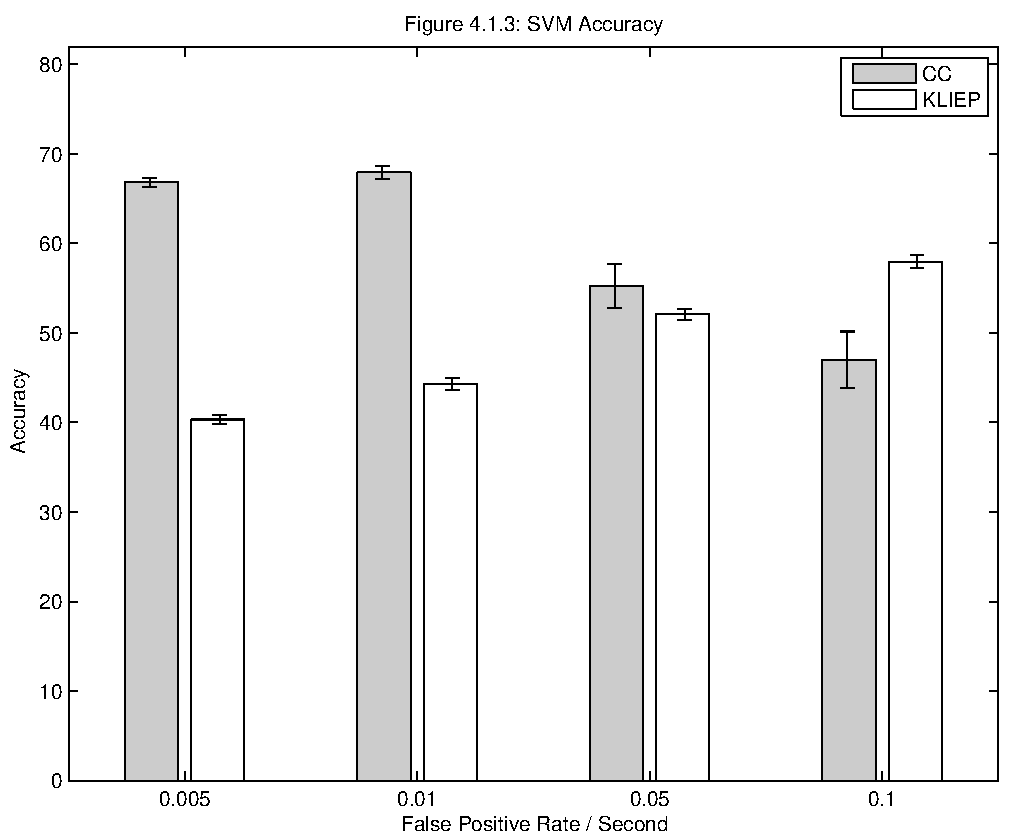
\includegraphics[scale=0.4]{osu_cpd_svm_acc.pdf} \hspace{1em}\vspace{1em}
 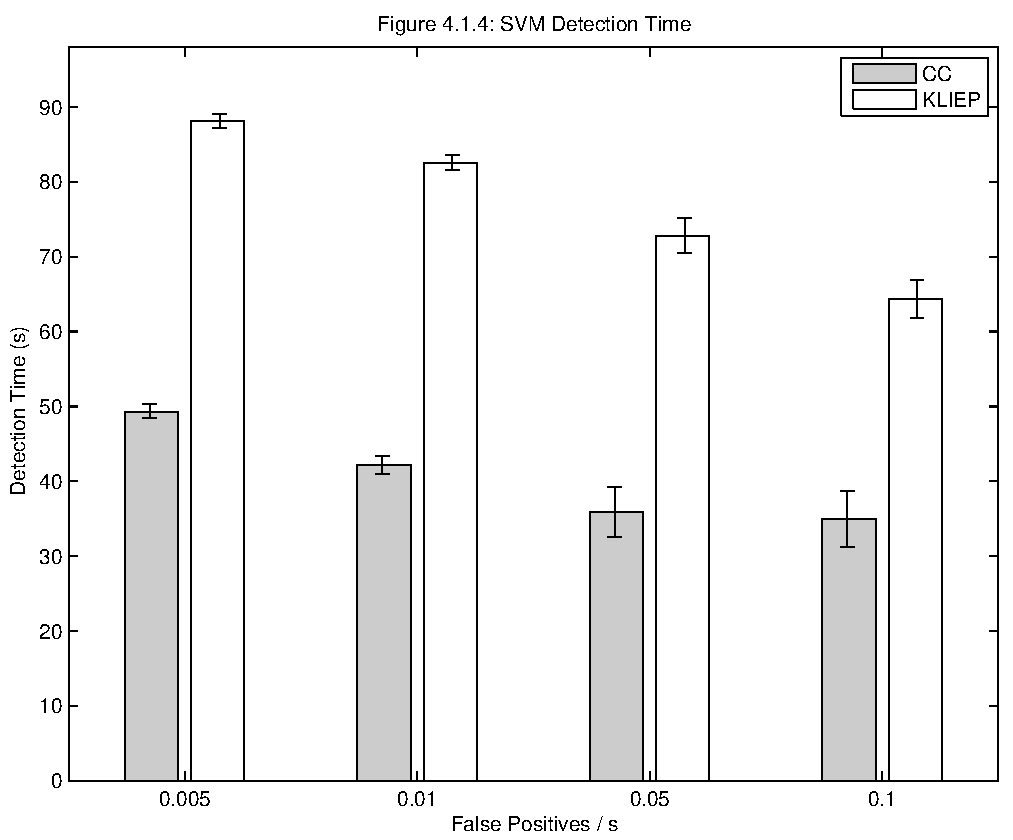
\includegraphics[scale=0.4]{osu_cpd_svm_det.pdf}
 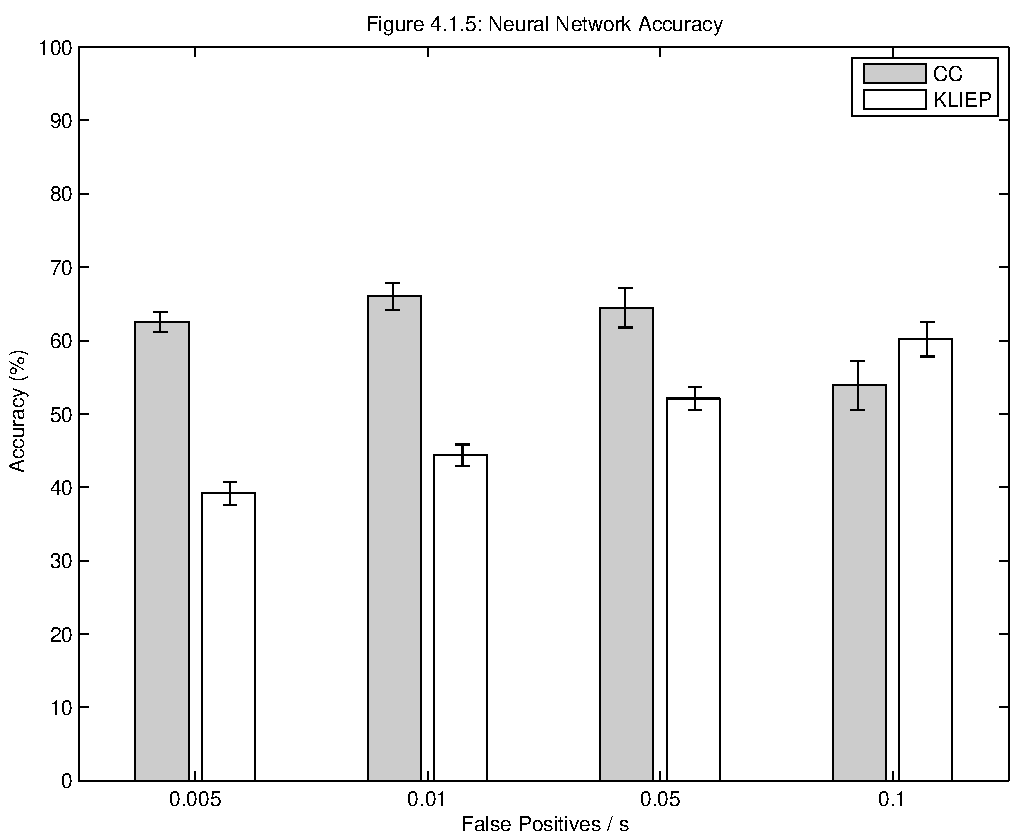
\includegraphics[scale=0.4]{osu_cpd_nnet_acc.pdf} \hspace{2em}
 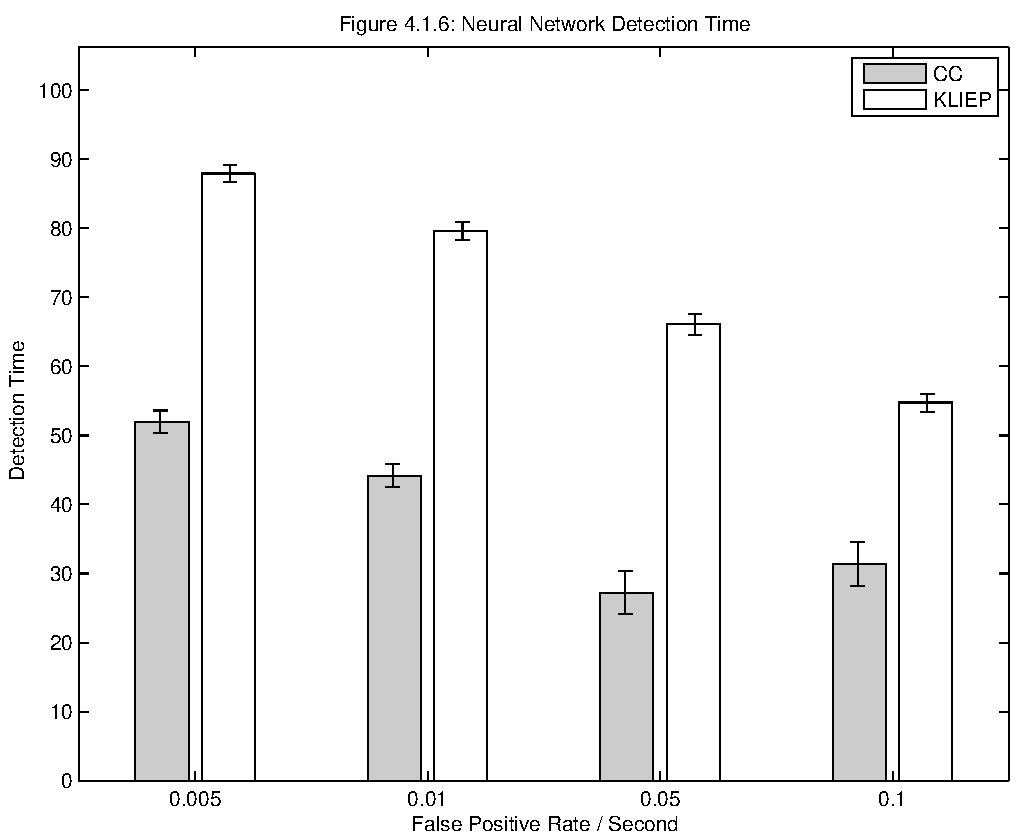
\includegraphics[scale=0.4]{osu_cpd_nnet_det.pdf}
 \caption{OSU Hip Results. Graphs are organized into rows by base classifier,
  and columns by evaluation metric. Change-point detection results were averaged over
  30 splits into training, testing, and validation datasets,
  along with error bars showing a 95\% confidence interval.}
 \label{fig:osu_cpd}
\end{figure}

\begin{figure}[H]
 \centering
 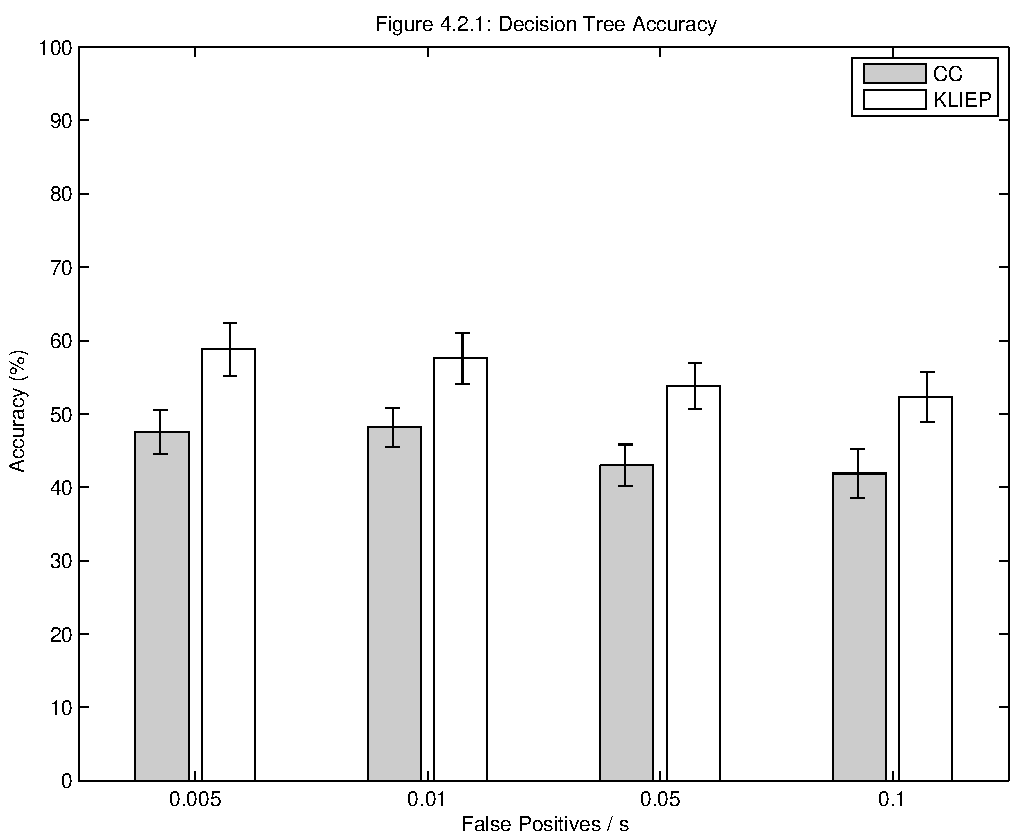
\includegraphics[scale=0.4]{lime1_cpd_dt_acc.pdf} \hspace{1em}\vspace{1em}
 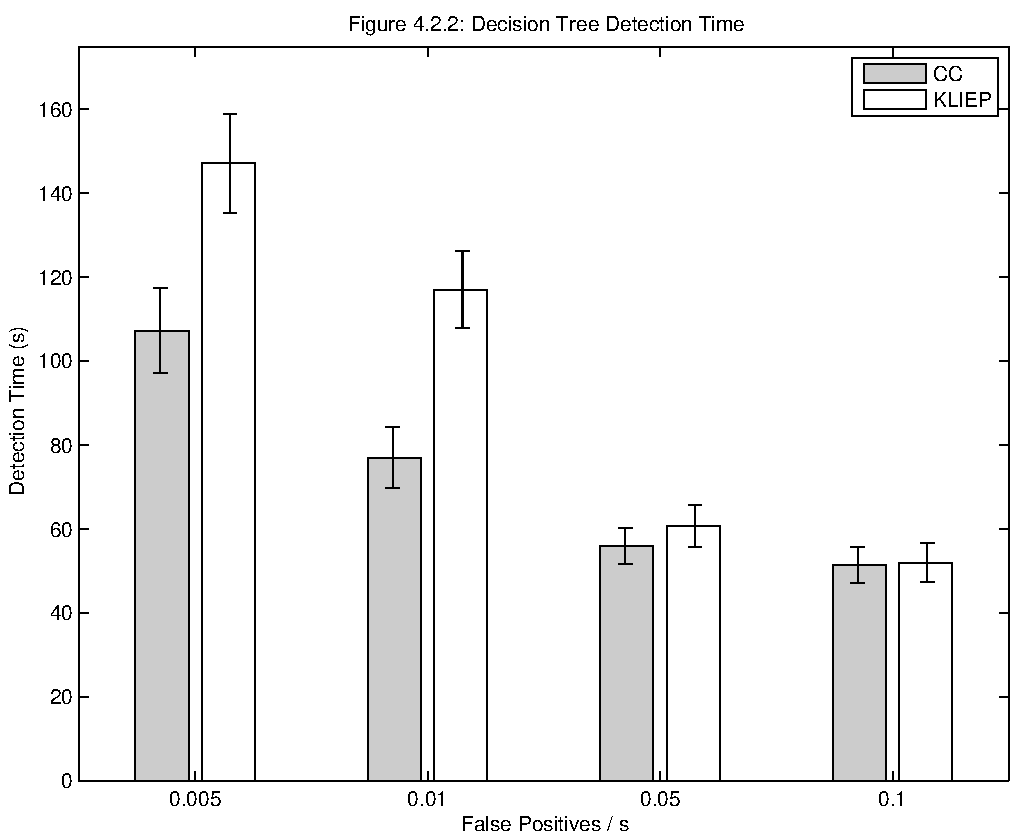
\includegraphics[scale=0.4]{lime1_cpd_dt_det.pdf}
 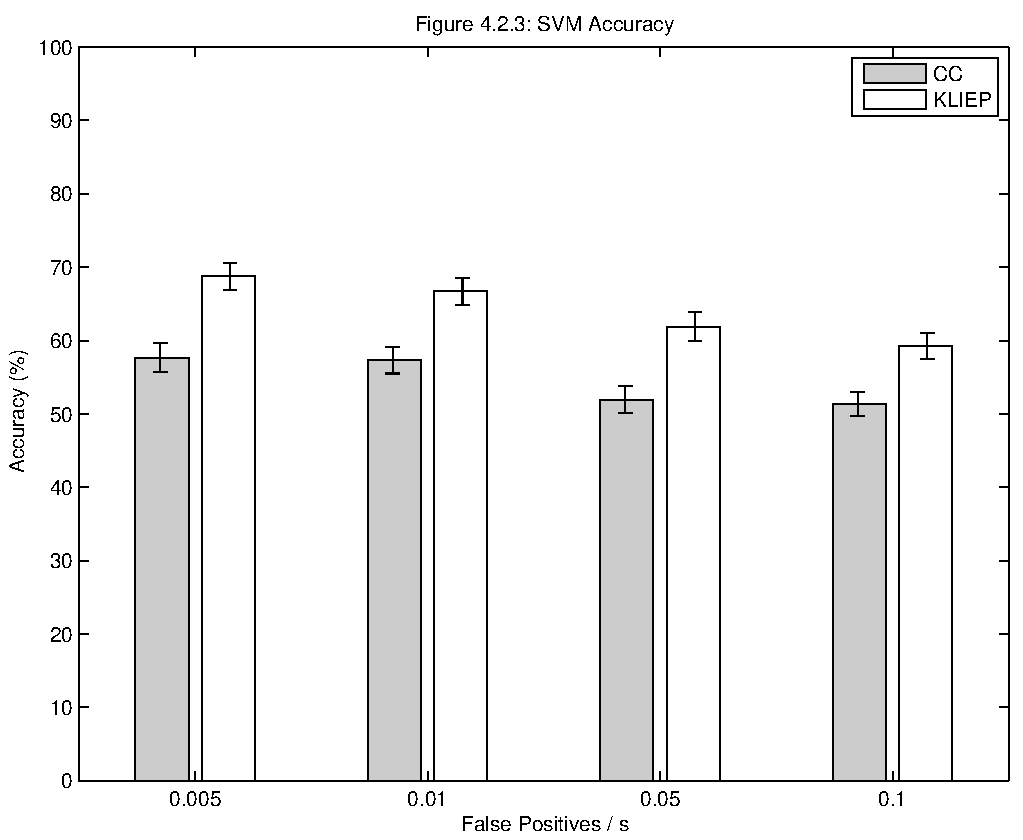
\includegraphics[scale=0.4]{lime1_cpd_svm_acc.pdf} \hspace{1em}\vspace{1em}
 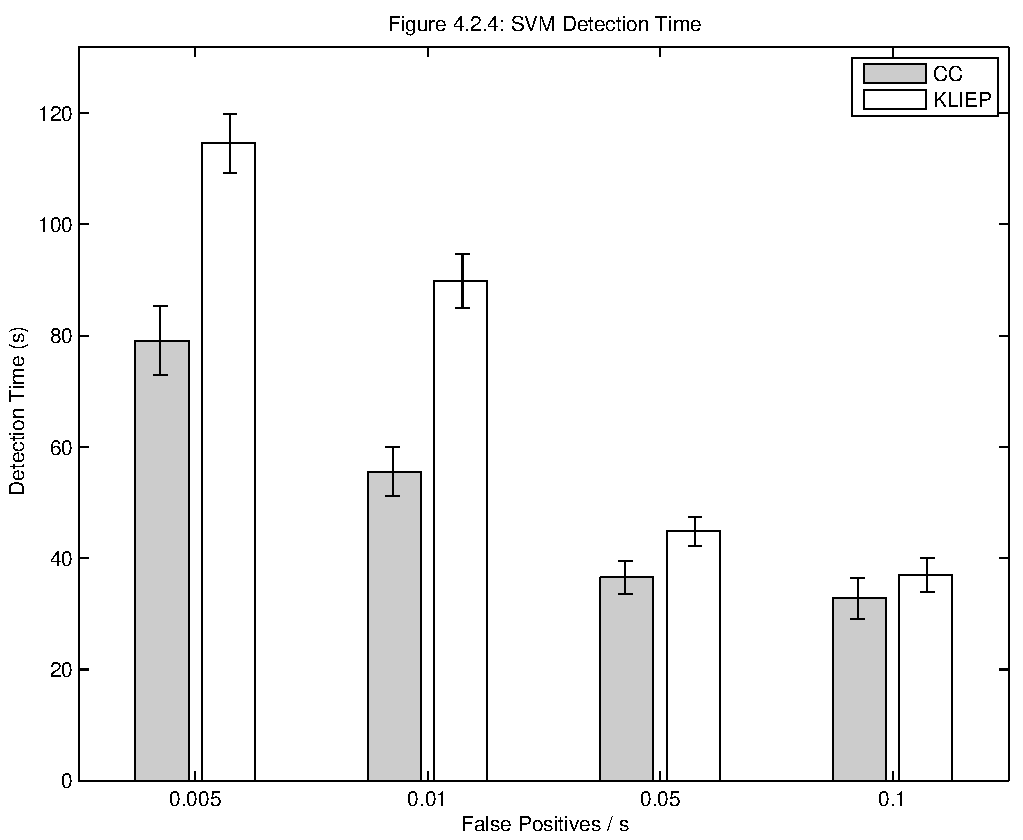
\includegraphics[scale=0.4]{lime1_cpd_svm_det.pdf}
 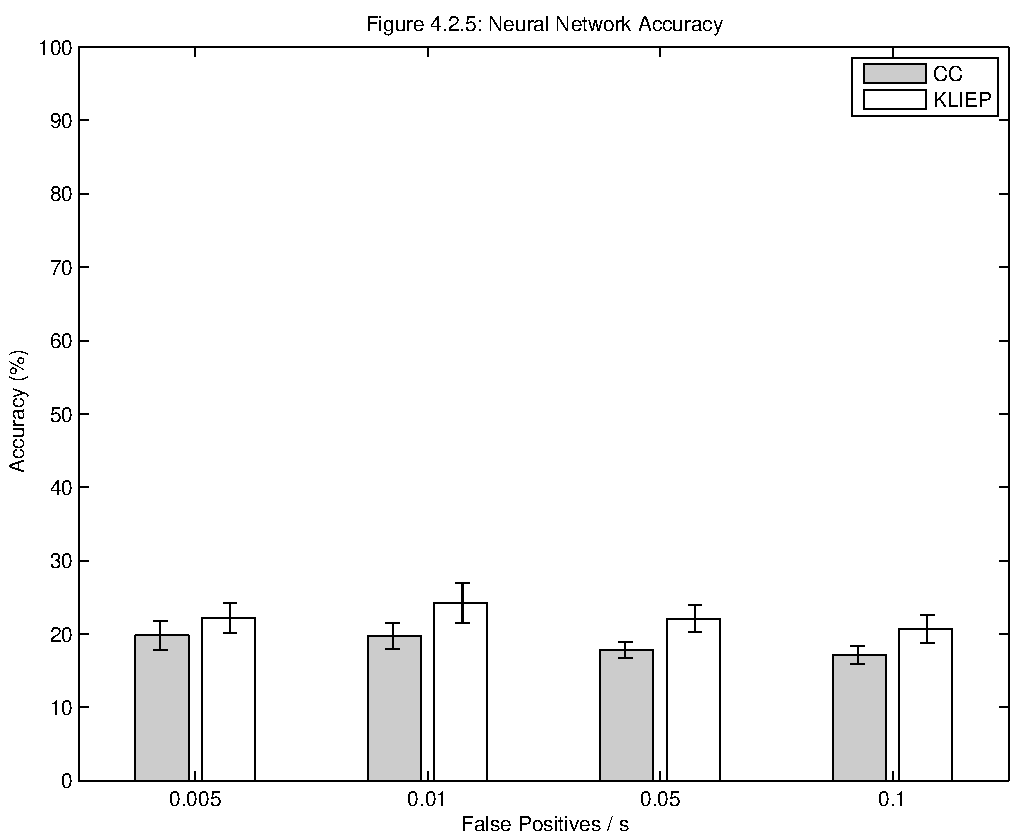
\includegraphics[scale=0.4]{lime1_cpd_nnet_acc.pdf} \hspace{1em}
 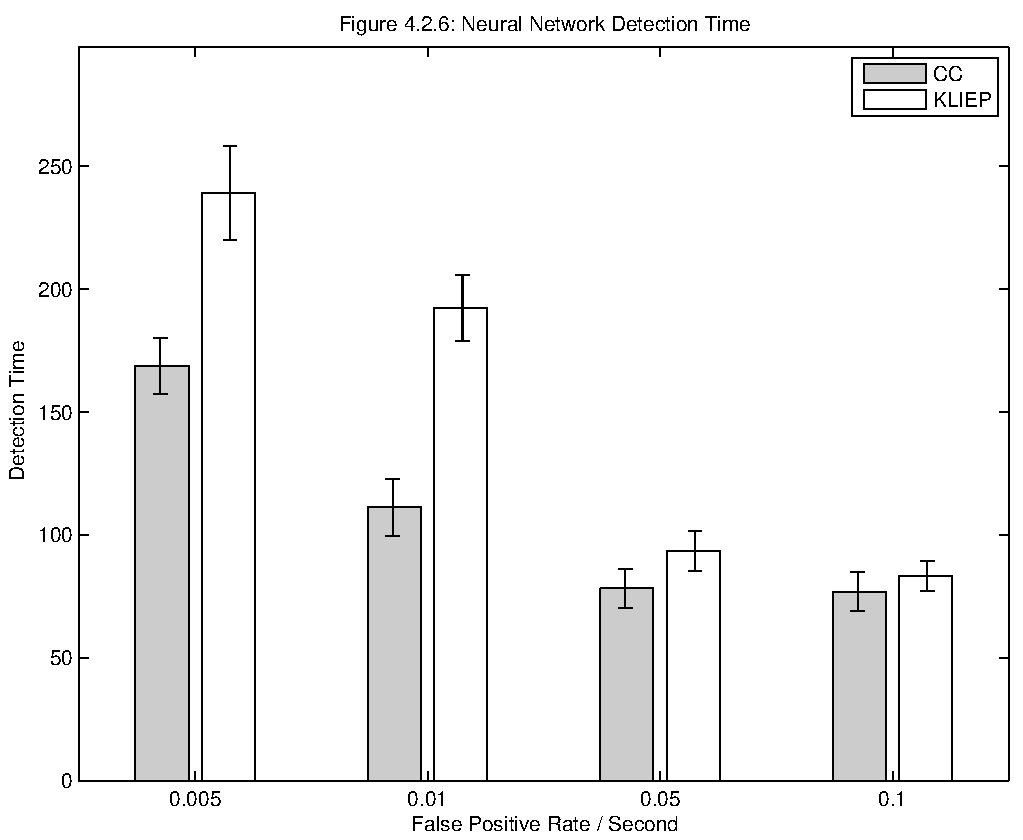
\includegraphics[scale=0.4]{lime1_cpd_nnet_det.pdf}
 \caption{LiME Day 1 Results. Graphs are organized into rows by base classifier,
  and columns by evaluation metric. Change-point detection results were averaged over
  30 splits into training, testing, and validation datasets,
  along with error bars showing a 95\% confidence interval.}
 \label{fig:lime1_cpd}
\end{figure}

\begin{figure}[H]
 \centering
 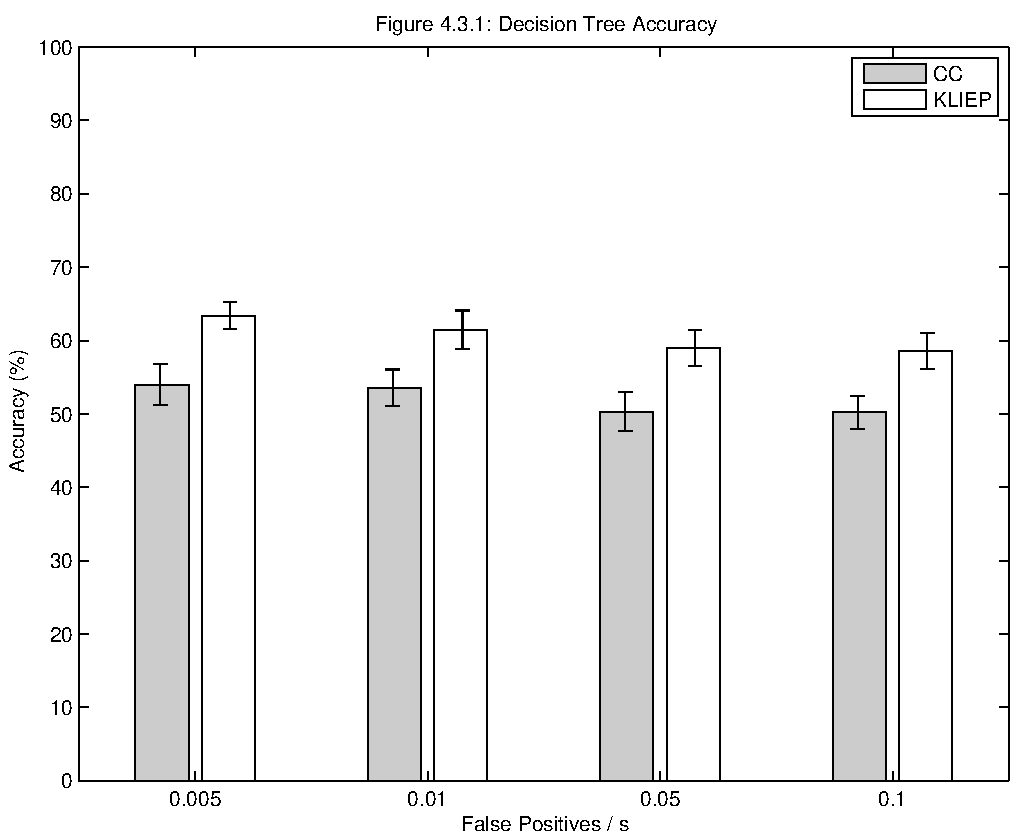
\includegraphics[scale=0.4]{lime2_cpd_dt_acc.pdf} \hspace{1em}\vspace{1em}
 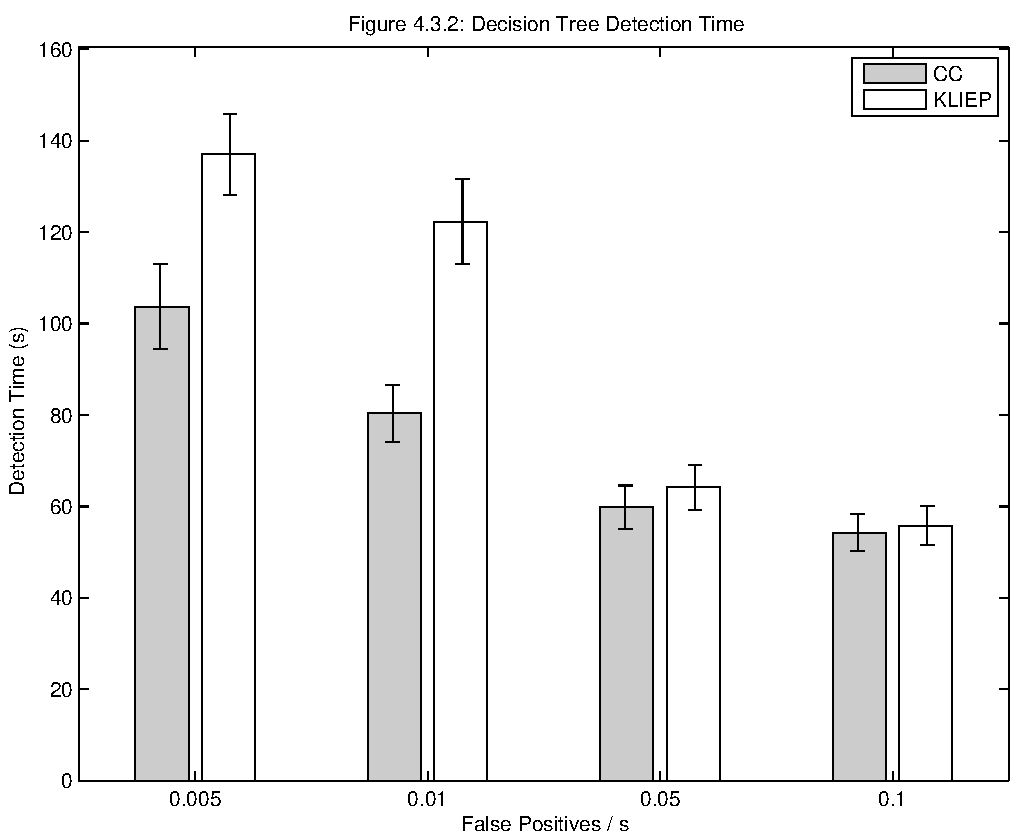
\includegraphics[scale=0.4]{lime2_cpd_dt_det.pdf}
 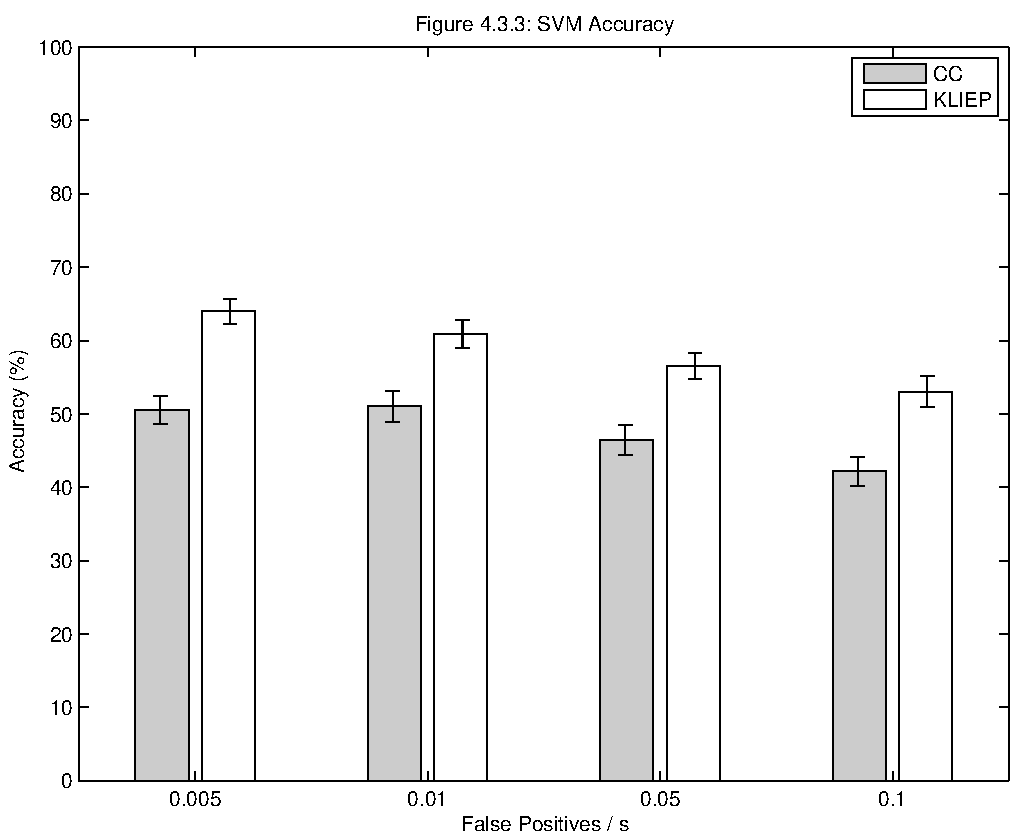
\includegraphics[scale=0.4]{lime2_cpd_svm_acc.pdf} \hspace{1em}\vspace{1em}
 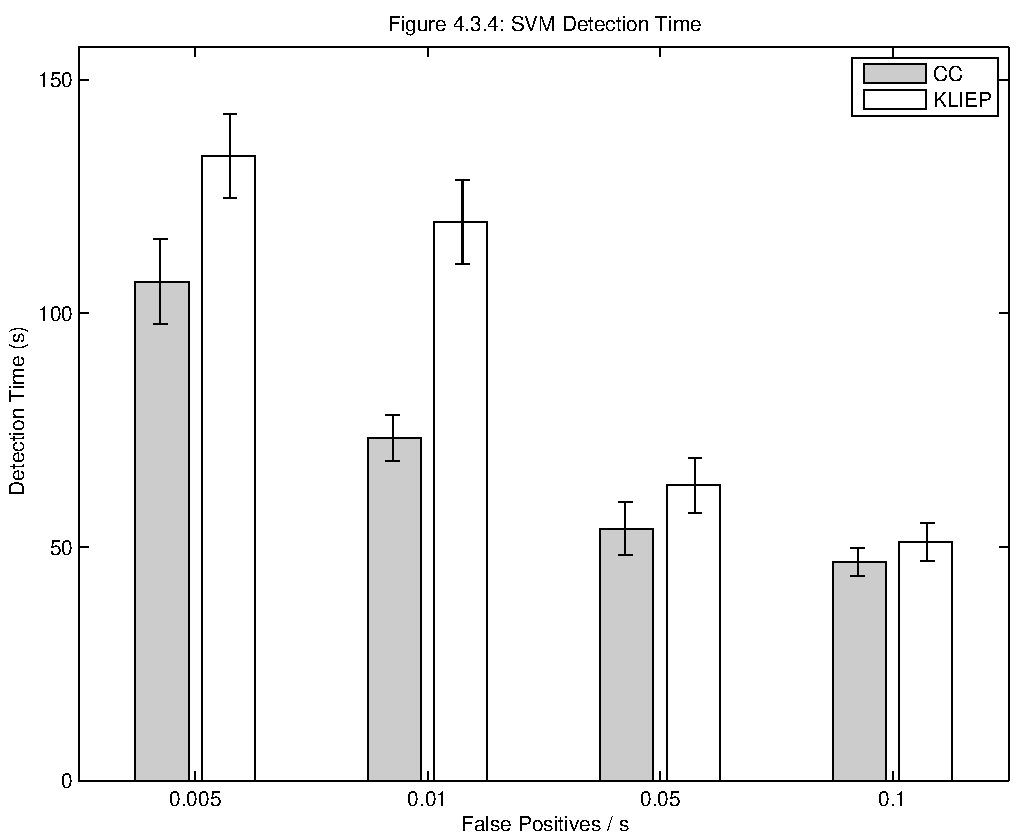
\includegraphics[scale=0.4]{lime2_cpd_svm_det.pdf}
 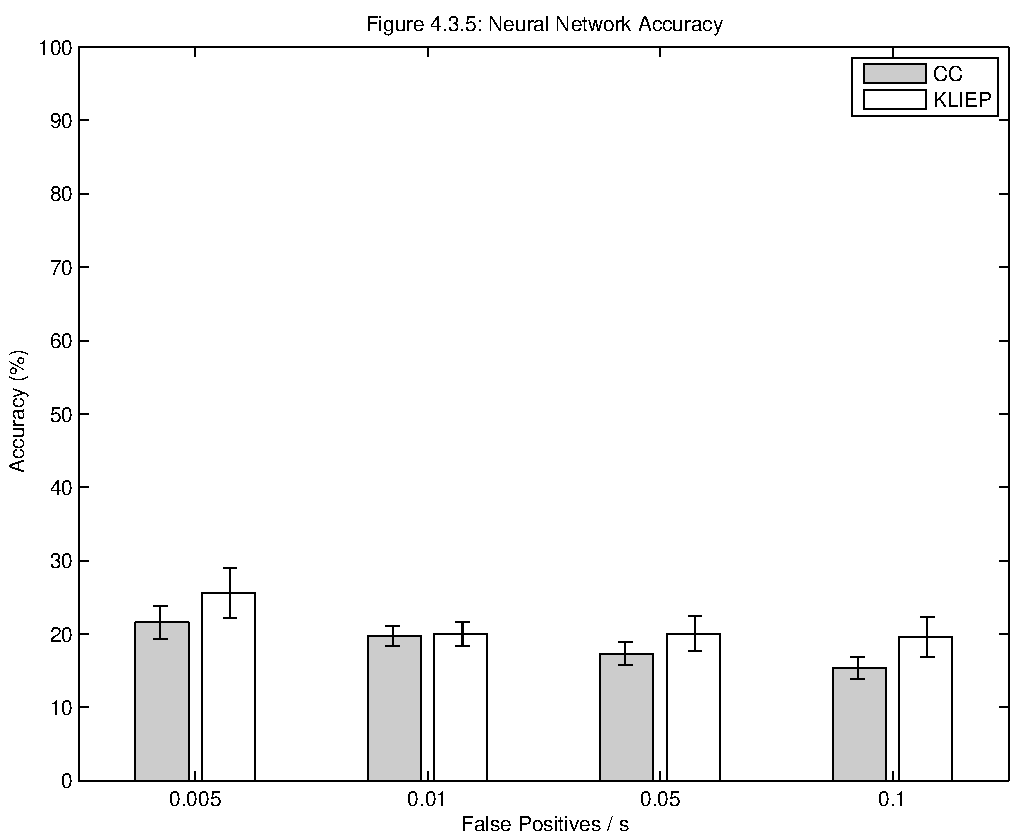
\includegraphics[scale=0.4]{lime2_cpd_nnet_acc.pdf} \hspace{1em}
 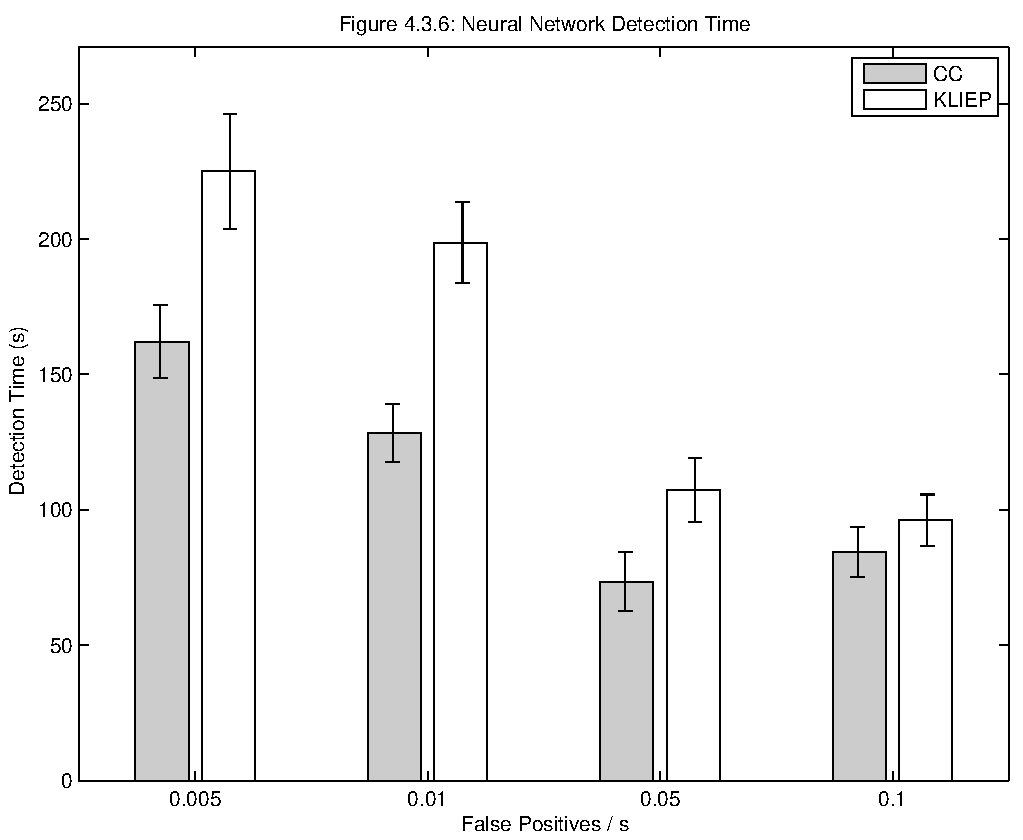
\includegraphics[scale=0.4]{lime2_cpd_nnet_det.pdf}
 \caption{LiME Day 2 Results. Graphs are organized into rows by base classifier,
  and columns by evaluation metric. Change-point detection results were averaged over
  30 splits into training, testing, and validation datasets,
  along with error bars showing a 95\% confidence interval.}
 \label{fig:lime2_cpd}
\end{figure}


\section{HMM}

Results for our HMM experiments are given in
Figures \ref{fig:osu_hmm}-\ref{fig:lime2_hmm}. Each HMM experiment was
performed by splitting each time series into windows of fixed length
corresponding to discrete time ``ticks'' in an HMM,
and results for windows of length $\{10, 12, 14, 16, 18, 20\}$
seconds are shown.

For both the SVM and decision tree classifiers, accuracy was high and
detection time was low across all three datasets. Accuracy and detection
time were also stable with respect to window size. Further experiments on the
OSU Hip dataset showed that the HMM when paired with these classifiers
tends to be stable with window sizes that are greater than a few seconds,
which seems to be the amount of time required to be informative. Neural networks
performed somewhat more poorly and erratically across the board.

\begin{figure}[H]
 \centering
 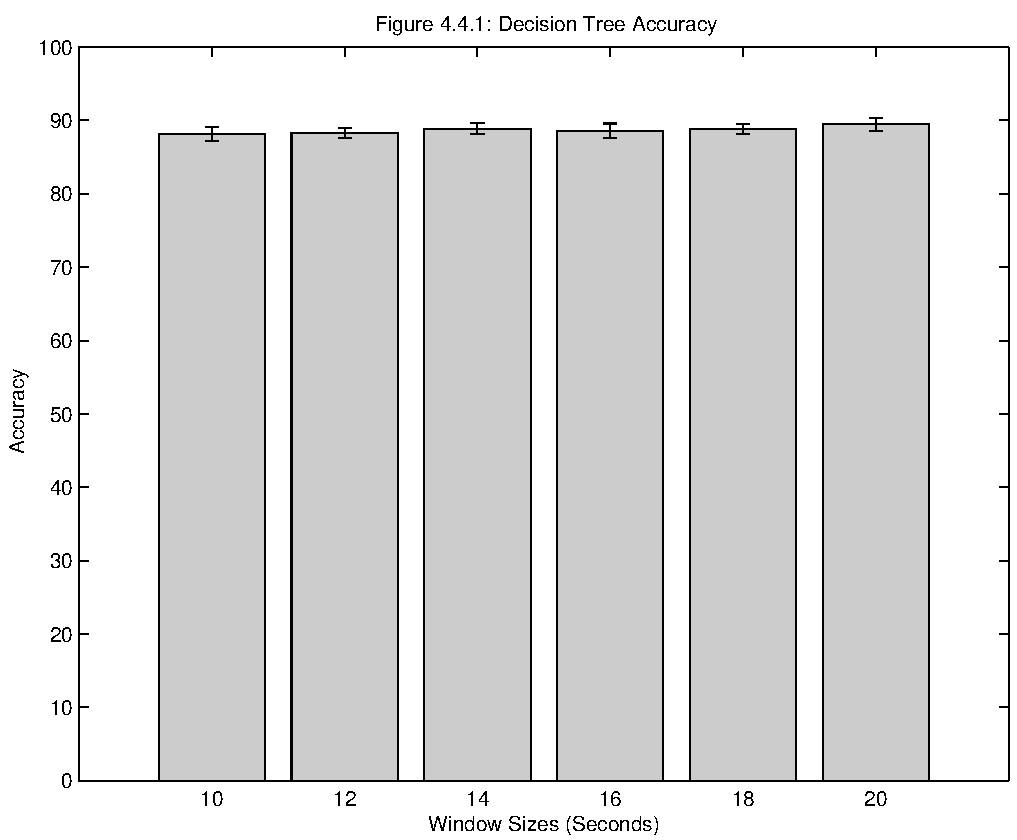
\includegraphics[scale=0.4]{osu_hmm_dt_acc.pdf} \hspace{1em}\vspace{1em}
 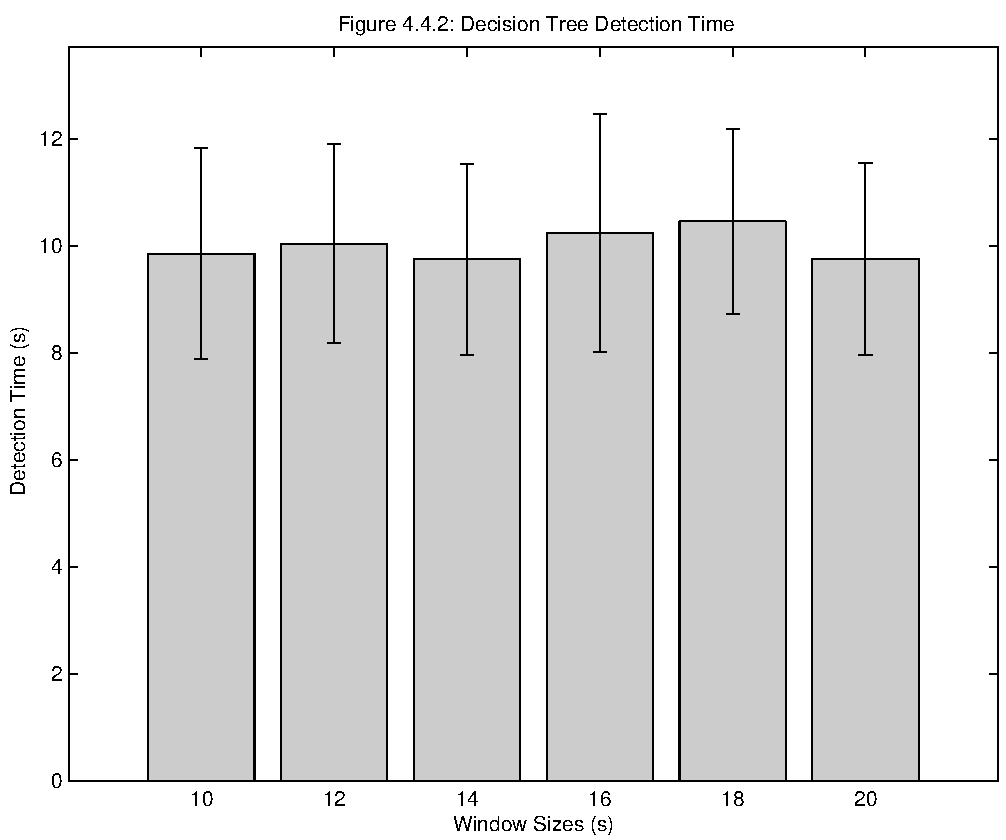
\includegraphics[scale=0.4]{osu_hmm_dt_det.pdf}
 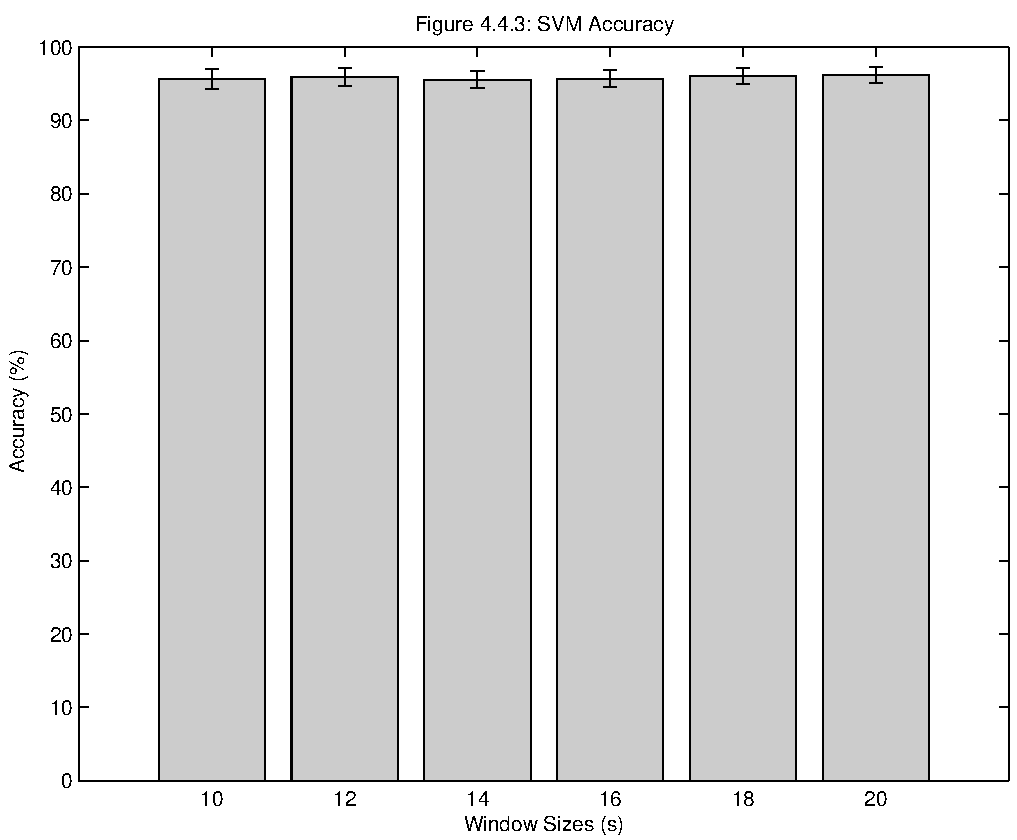
\includegraphics[scale=0.4]{osu_hmm_svm_acc.pdf} \hspace{1em}\vspace{1em}
 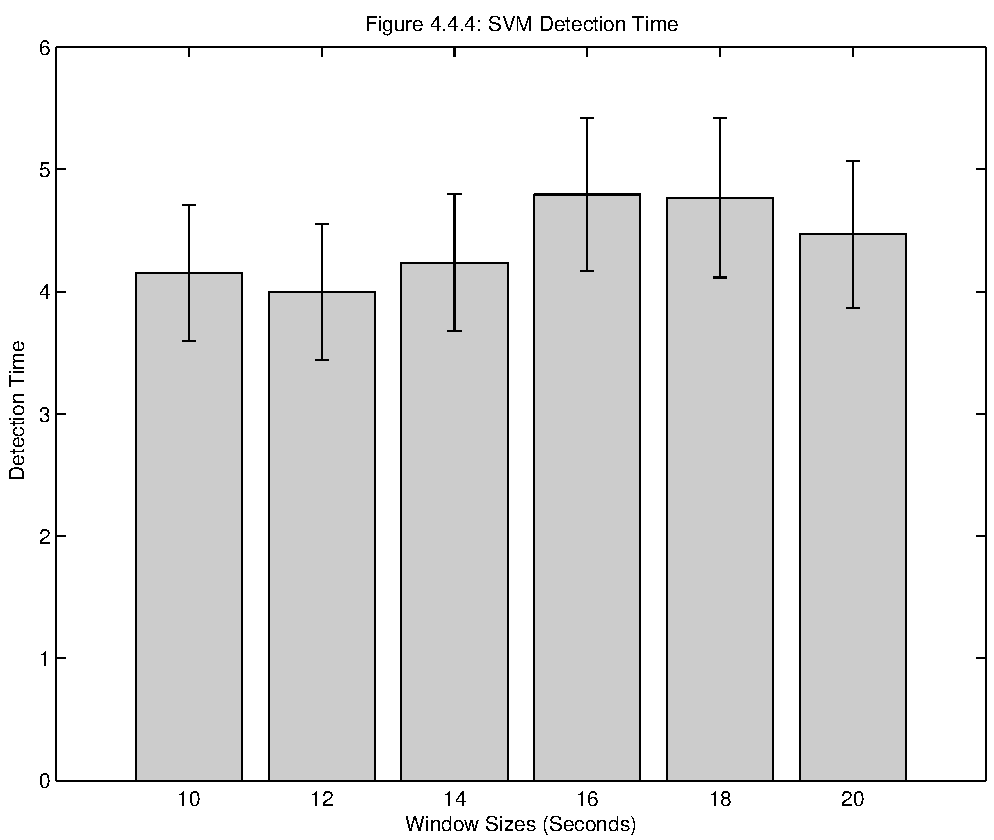
\includegraphics[scale=0.4]{osu_hmm_svm_det.pdf}
 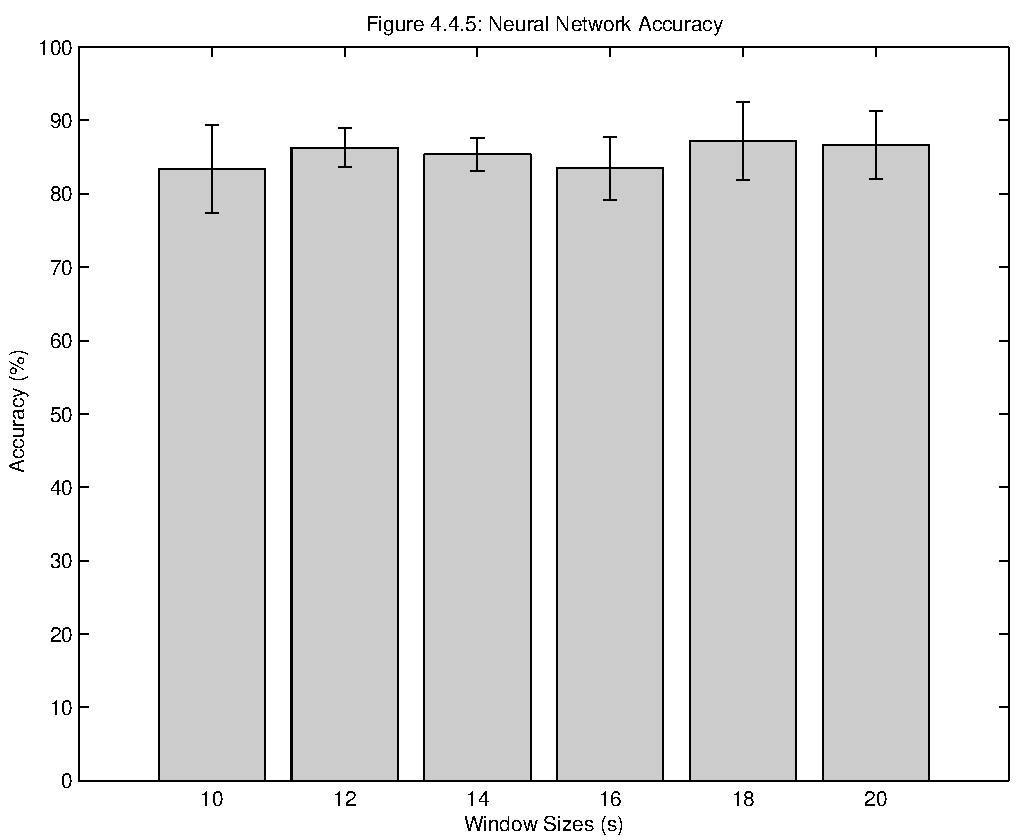
\includegraphics[scale=0.4]{osu_hmm_nnet_acc.pdf} \hspace{1em}
 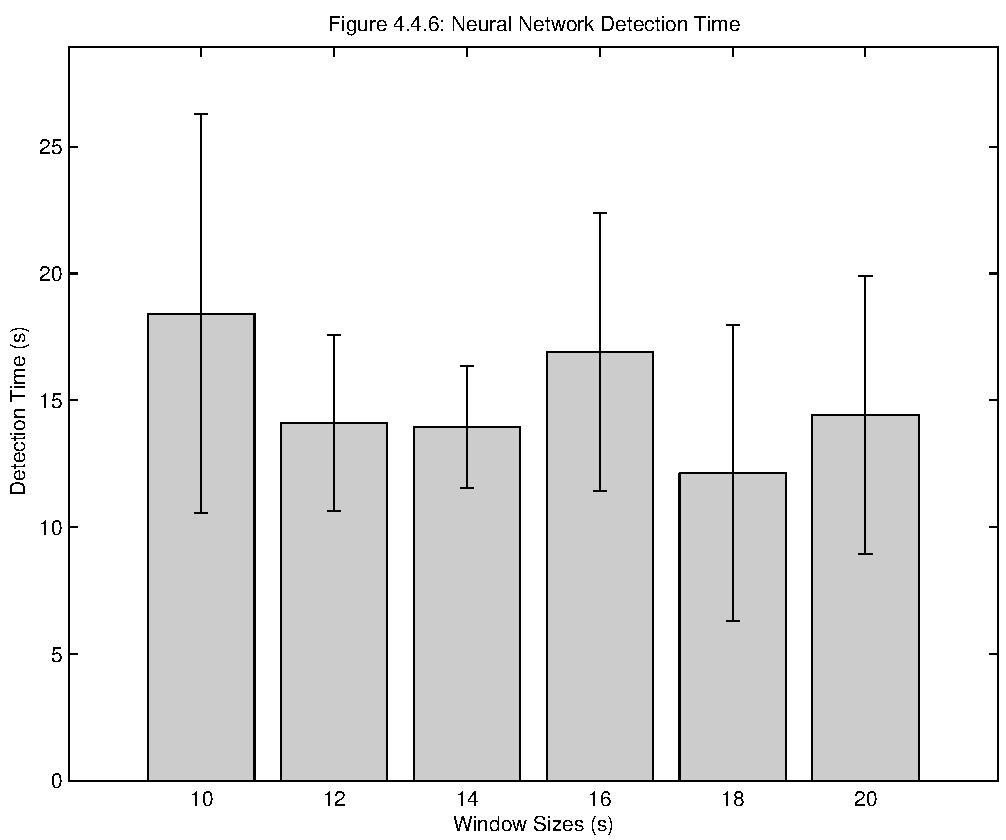
\includegraphics[scale=0.4]{osu_hmm_nnet_det.pdf}
 \caption{OSU Hip HMM Results.
  Graphs are organized into rows by base classifier, and columns by evaluation
  metric. HMM results were averaged over 10 splits into training
  (base classifier), validation, training (HMM), and testing datasets, along with 
  error bars showing a 95\% confidence interval.}
 \label{fig:osu_hmm}
\end{figure}

\begin{figure}[H]
 \centering
 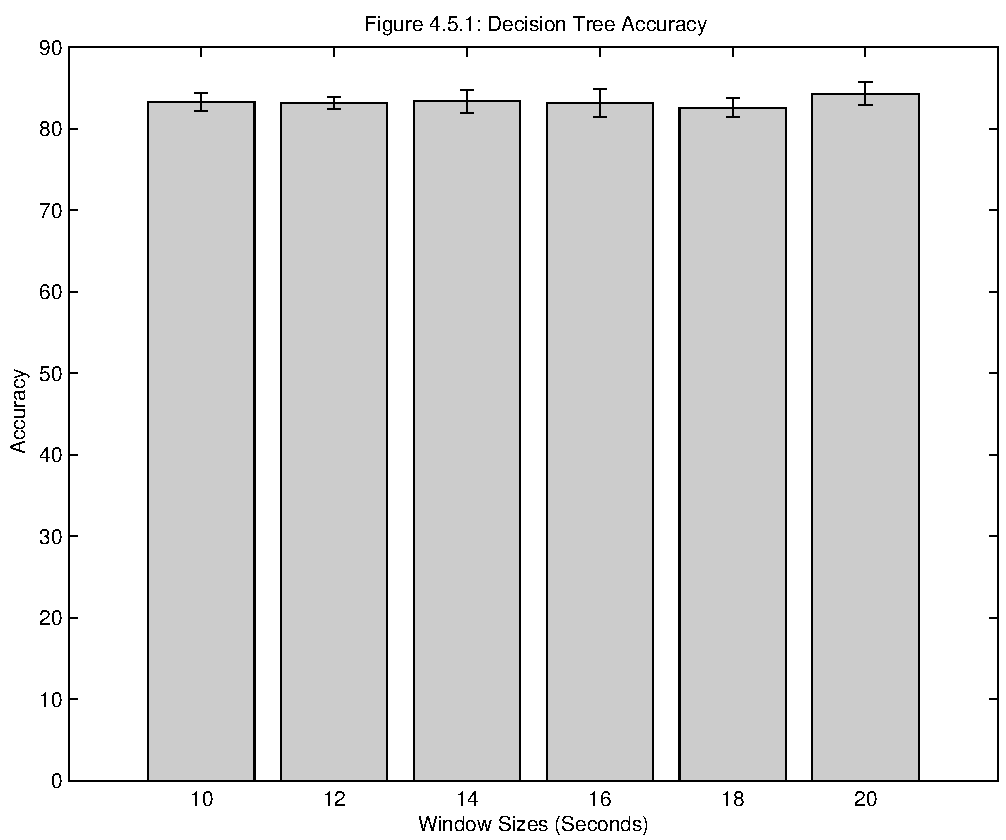
\includegraphics[scale=0.4]{lime1_hmm_dt_acc.pdf} \hspace{1em}\vspace{1em}
 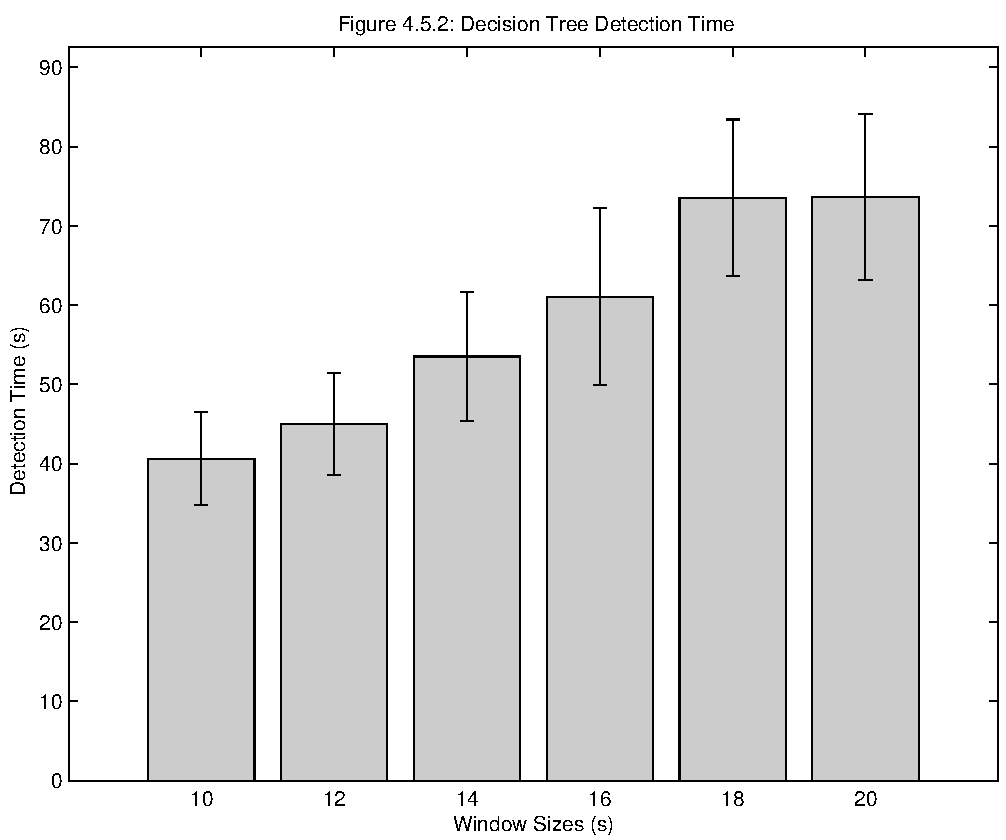
\includegraphics[scale=0.4]{lime1_hmm_dt_det.pdf} 
 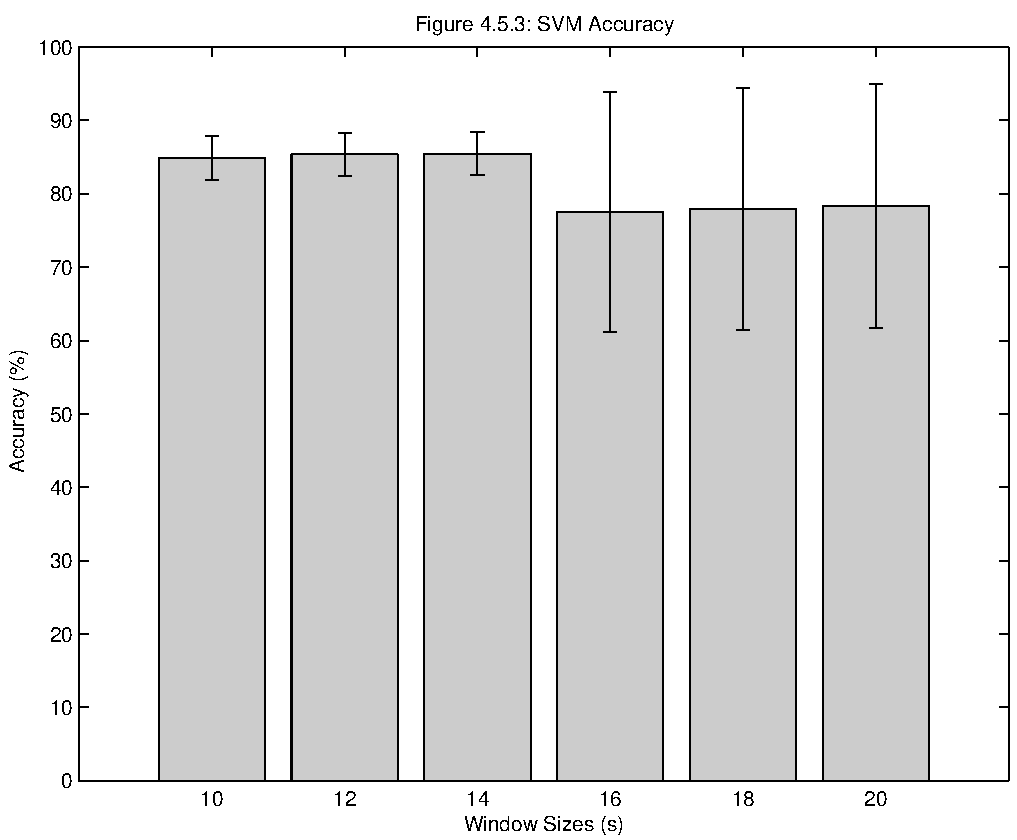
\includegraphics[scale=0.4]{lime1_hmm_svm_acc.pdf} \hspace{1em}\vspace{1em}
 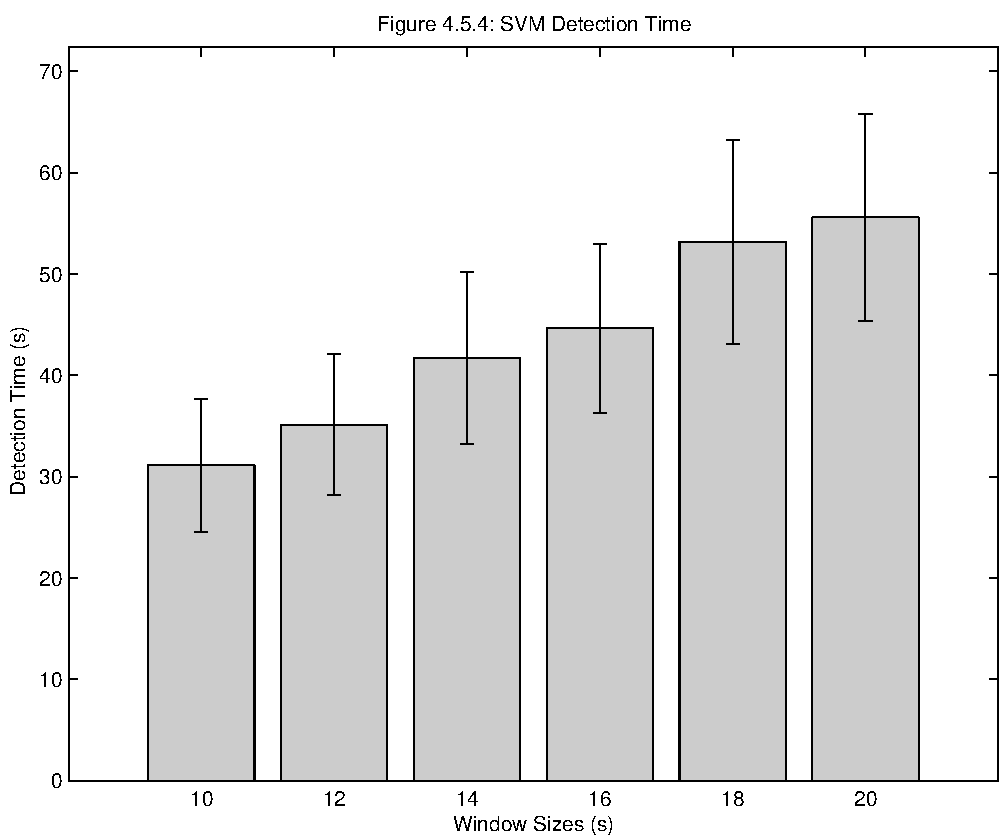
\includegraphics[scale=0.4]{lime1_hmm_svm_det.pdf} 
 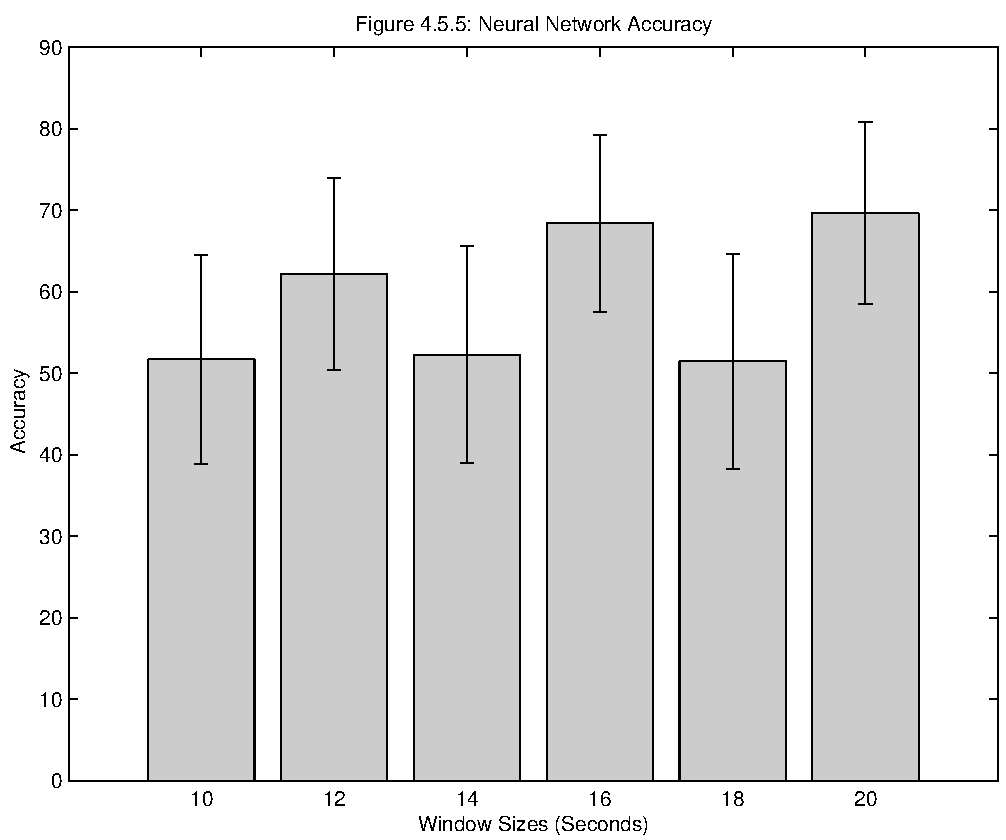
\includegraphics[scale=0.4]{lime1_hmm_nnet_acc.pdf} \hspace{1em}
 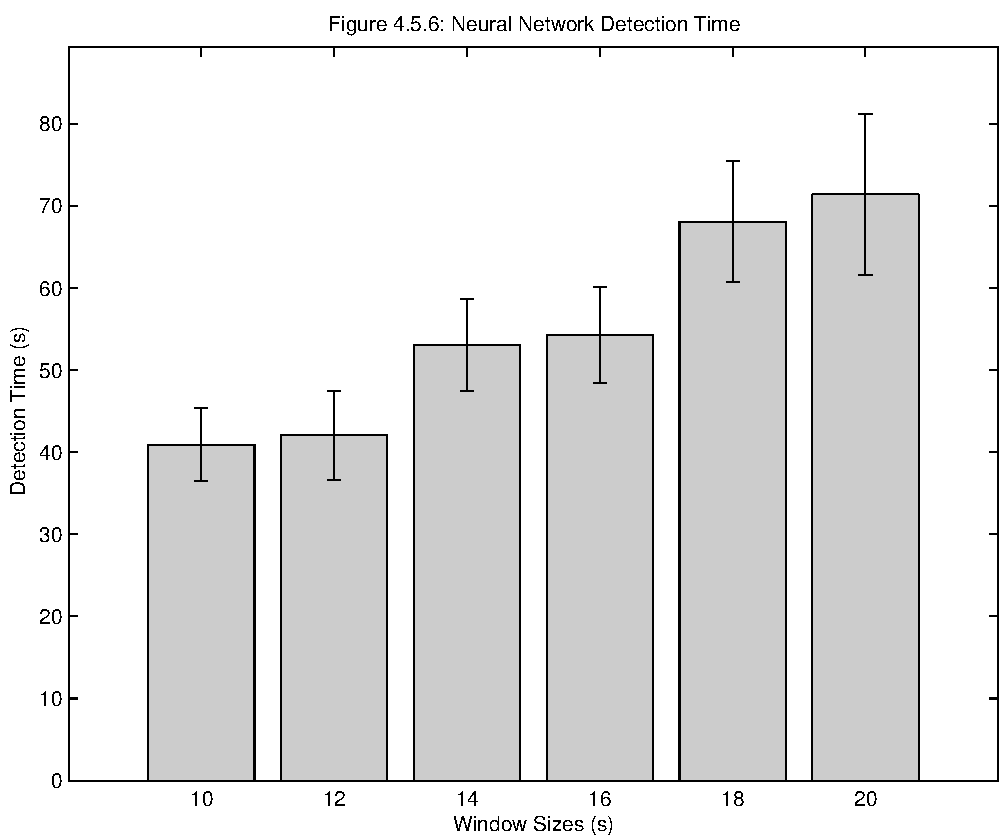
\includegraphics[scale=0.4]{lime1_hmm_nnet_det.pdf} 
 \caption{LiME Day 1 HMM Results.
  Graphs are organized into rows by base classifier, and columns by evaluation
  metric. HMM results were averaged over 10 splits into training
  (base classifier), validation, training (HMM), and testing datasets, along with 
  error bars showing a 95\% confidence interval.}
 \label{fig:lime1_hmm}
\end{figure}

\begin{figure}[H]
 \centering
 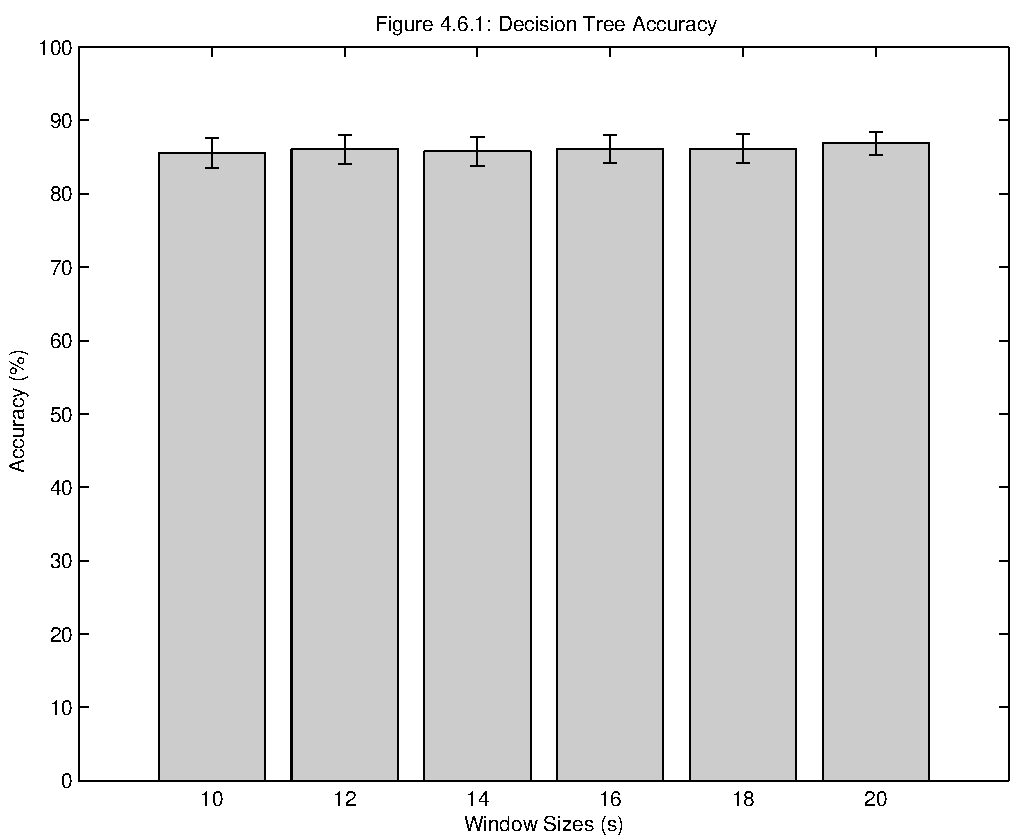
\includegraphics[scale=0.4]{lime2_hmm_dt_acc.pdf} \hspace{1em}\vspace{1em}
 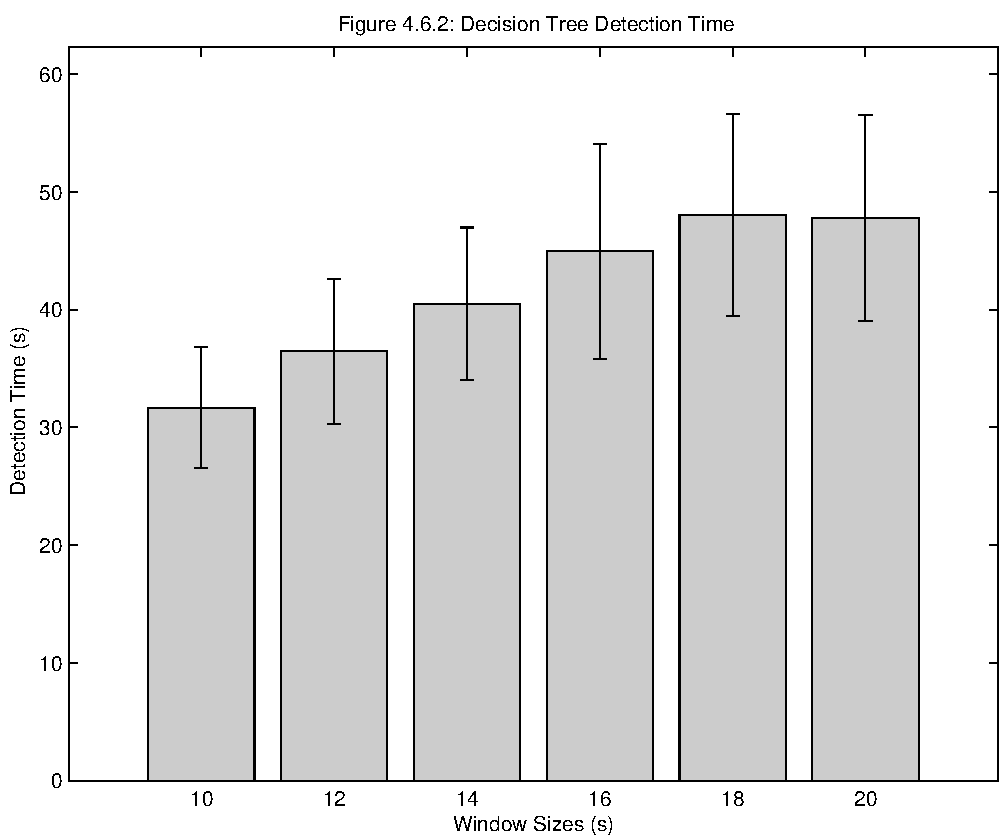
\includegraphics[scale=0.4]{lime2_hmm_dt_det.pdf}
 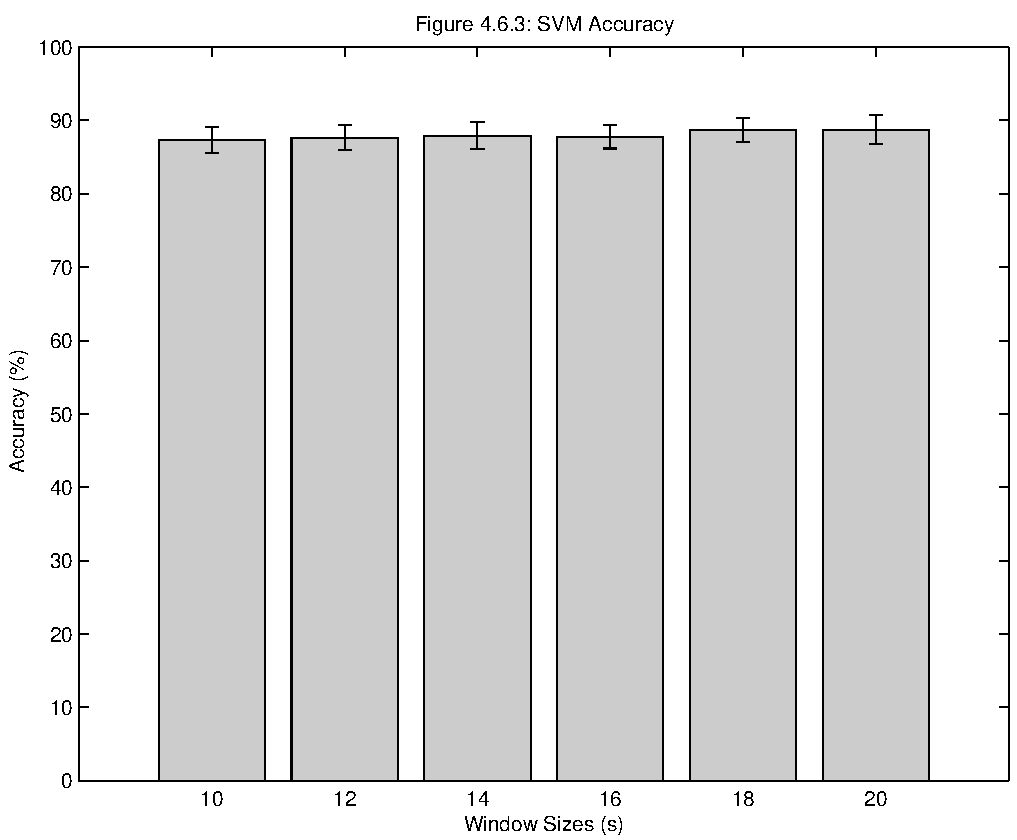
\includegraphics[scale=0.4]{lime2_hmm_svm_acc.pdf} \hspace{1em}\vspace{1em}
 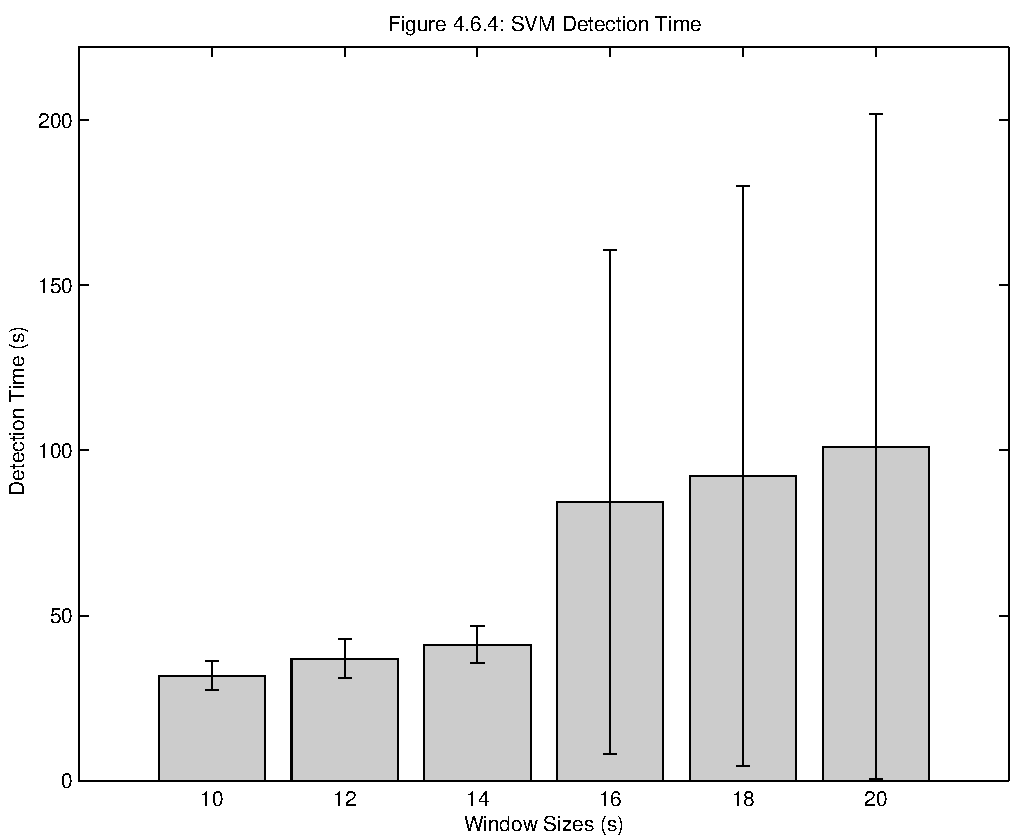
\includegraphics[scale=0.4]{lime2_hmm_svm_det.pdf}
 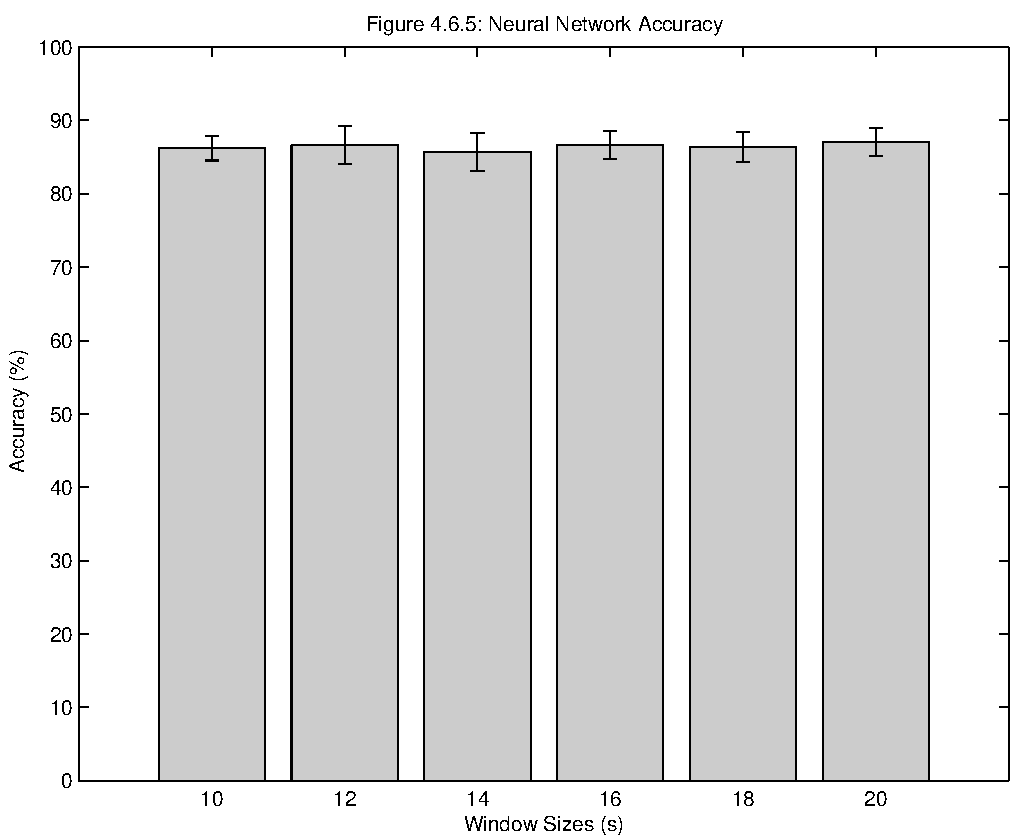
\includegraphics[scale=0.4]{lime2_hmm_nnet_acc.pdf} \hspace{1em}
 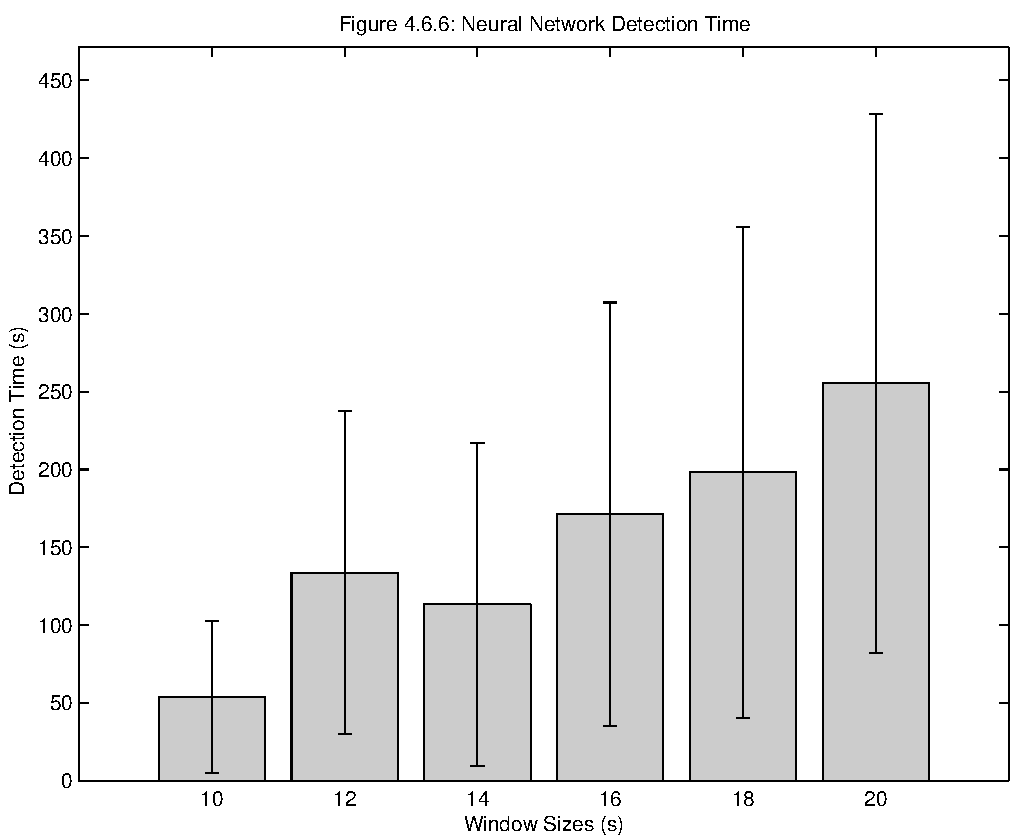
\includegraphics[scale=0.4]{lime2_hmm_nnet_det.pdf}
 \caption{LiME Day 2 HMM Results.
  Graphs are organized into rows by base classifier, and columns by evaluation
  metric. HMM results were averaged over 10 splits into training
  (base classifier), validation, training (HMM), and testing datasets, along with 
  error bars showing a 95\% confidence interval.}
 \label{fig:lime2_hmm}
\end{figure}

\newpage

\section{Discussion}

Our results clearly show that the HMM approach outperformed the change-point
detection approach, both in terms of accuracy and detection time, regardless of
the dataset and base classifier. Figure \ref{fig:compare_cpd_hmm} shows a
side-by-side comparison of the top-down and bottom-up approaches. 
HMMs likely did better because they are trained
on labelled data. Change-point detection algorithms on the other hand are unaware of
true activity labels---they merely signal a change when they detect a distance or
dissimilarity between reference and test data. As such, change-point detection
algorithms have trouble accurately segmenting free-living data, and noisy
segmentation results in poor performance.

A contributing factor to the particularly high accuracy and low detection time
results attained for the OSU Hip experiments was that the data consisted of
activities that were synthetically glued together. The same group of activities
were performed in the same order by each of the 50 subjects in this dataset,
making transitions from one activity to the other very predictable for a
temporal model. By contrast, the LiME datasets consisted of unsynthetic data
gathered from a large set of unstructured and variable-length activities,
so the activity transitions were not as predictable and are more indicative of
an application of our techniques in the real world.

%TODO (Compare LiME 1 with LiME 2 in this paragraph or the next one.)

A final point of interest was that SVM clearly outperformed the other two
base classifiers, and that the faster and simpler decision tree model did fairly
well against neural networks. This result is significant because much of the
previous research that has formulated activity detection as a supervised learning
problem has used neural networks exclusively.

\begin{figure}[h]
 \centering
 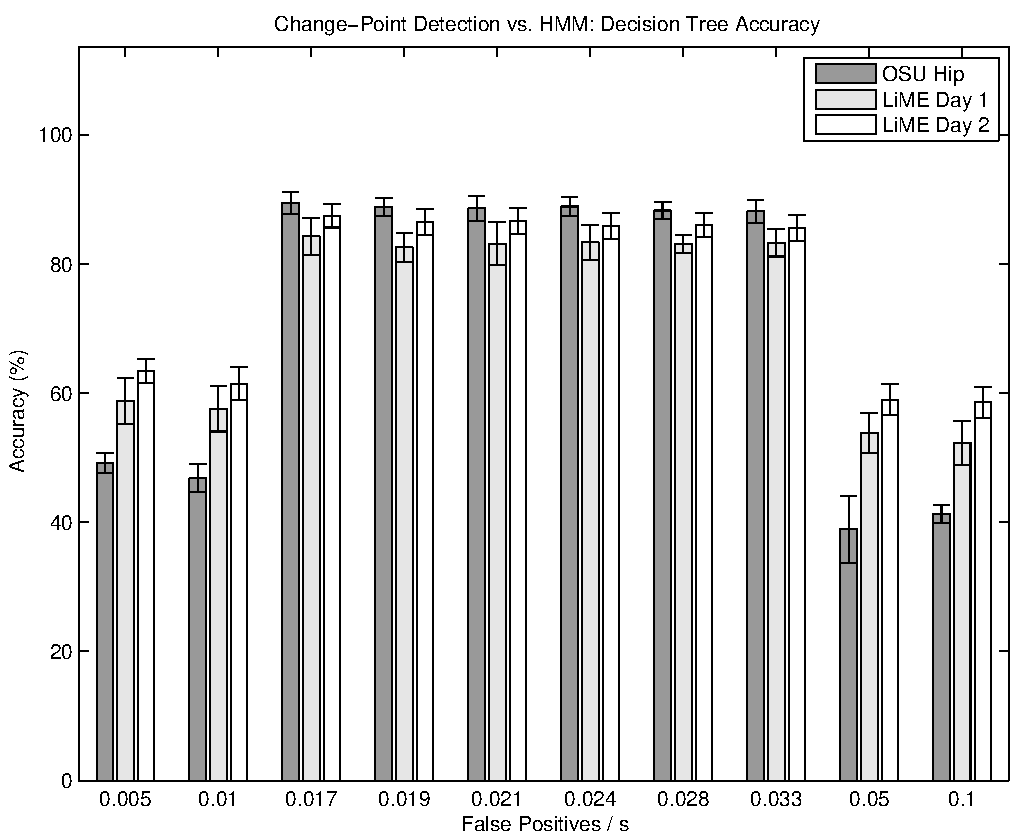
\includegraphics[scale=0.55]{cpd_hmm_compare_acc.pdf}
 
\includegraphics[scale=0.3]{vspace.png}
 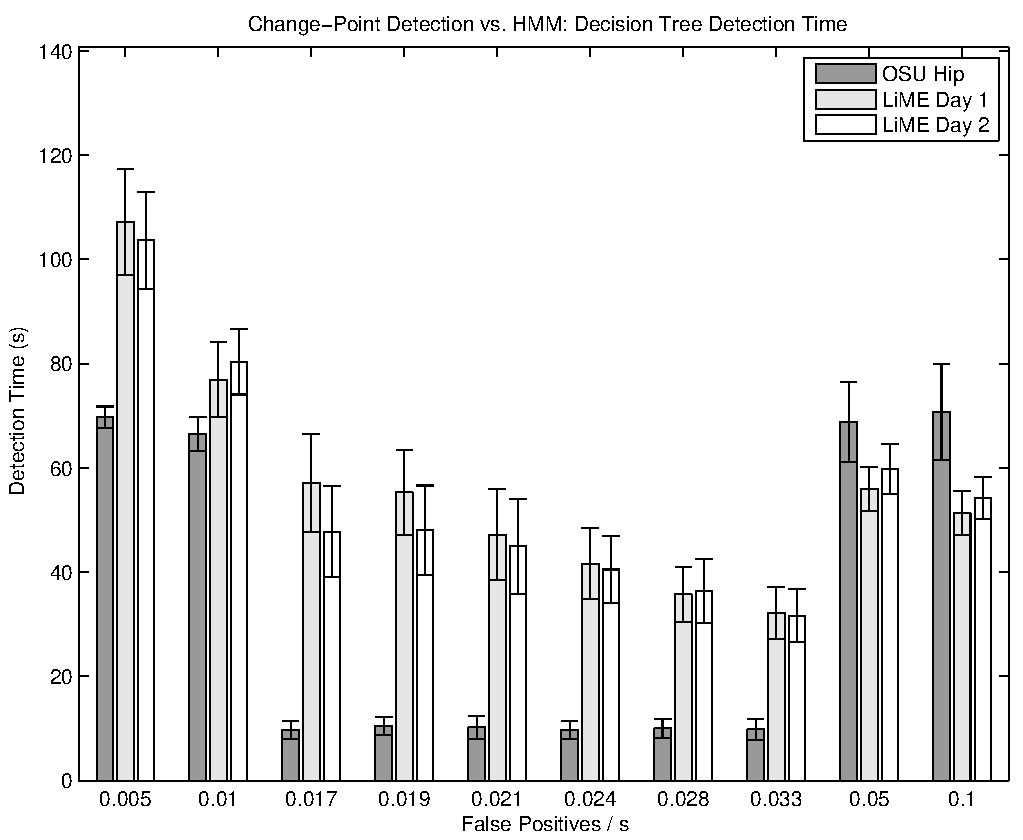
\includegraphics[scale=0.55]{cpd_hmm_compare_det.pdf}
 \caption{Comparison of change-point detection and HMMs in terms of accuracy
  and detection time. For a given false positive rate, change-point detection
  algorithms split a time series into windows of a certain average size, which
  decreases as the false positive rate increases. From this it is possible to relate
  false positive rates from the CPD experiments to the window sizes of the
  HMM experiments. Here is the HMM data with false positive rates of 
  \{0.033, 0.028, 0.024, 0.021, 0.019, 0.017\} that would
  correspond to average window sizes of \{10, 12, 14, 16, 18, 20\}. Both
  graphs show decision tree results, and both show results from each of the
  three datasets clustered together over a single false positive rate.}
 \label{fig:compare_cpd_hmm}
\end{figure}
